\lstinputlisting[language=bash,basicstyle=\small]{python_codes/fieldstone_78/keywords}

\begin{center}
Code at \url{https://github.com/cedrict/fieldstone/tree/master/python_codes/fieldstone_78}
\end{center}

\par\noindent\rule{\textwidth}{0.4pt}

%%%%%%%%%%%%%%%%%%%%%%%%%%%%%%%%%%%%%%%%%%%%%%%%%%%%%%%%%%%%%%%%%%%%%%%%%%%%%%%%%%%%%%%%%%%%%%%%%%%%


Although the $Q_1\times P_0$ is not LBB-stable (see Section~\ref{ss:LBBcond})
it has been proven that some spatial arrangements of this element can be, such as the
so-called Stenberg macro-element described in Section~\ref{ss:meshtopos}.
On the following a mesh is shown which consists of $16\times 16$ of such macro-elements:

\begin{center}
a)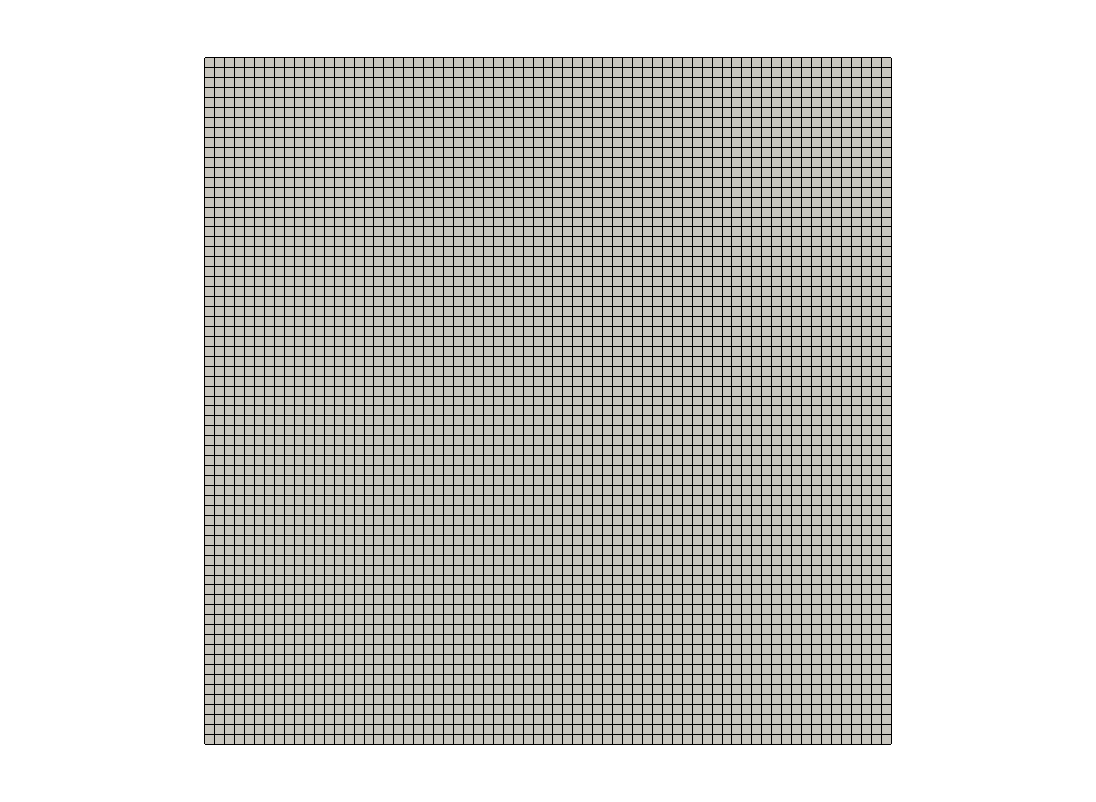
\includegraphics[width=7cm]{python_codes/fieldstone_78/results/mms/grid0}
b)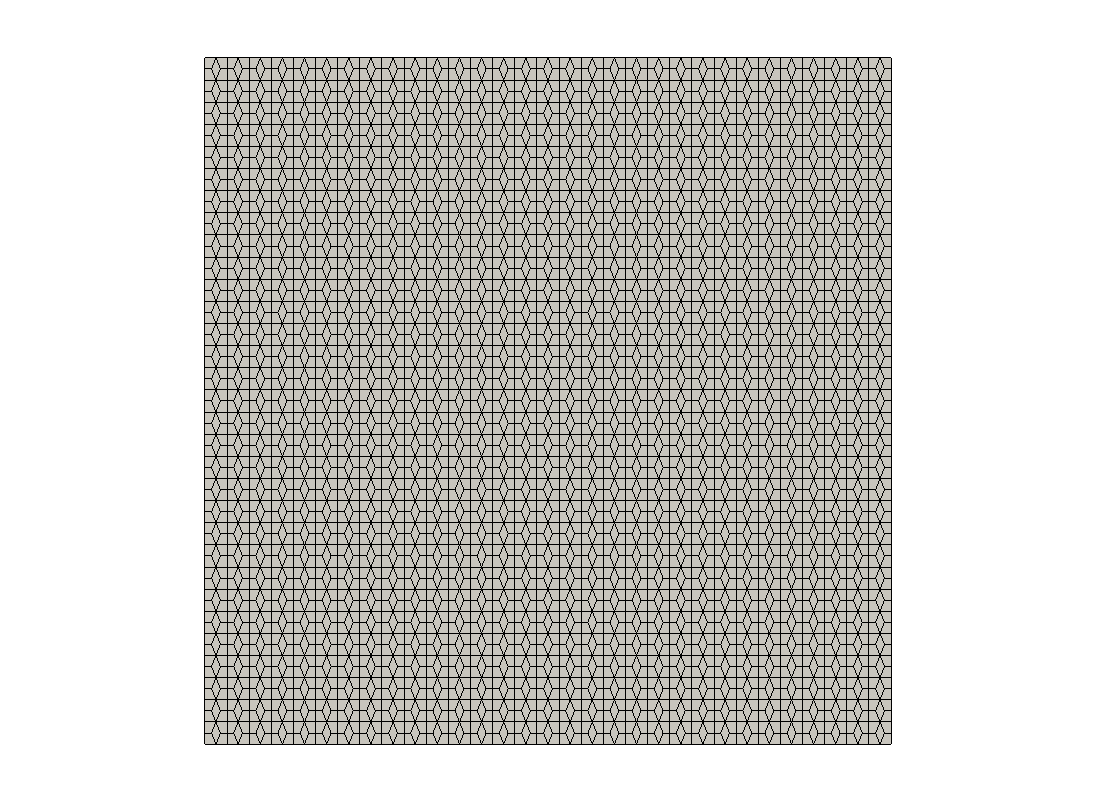
\includegraphics[width=7cm]{python_codes/fieldstone_78/results/mms/grid1}\\
c)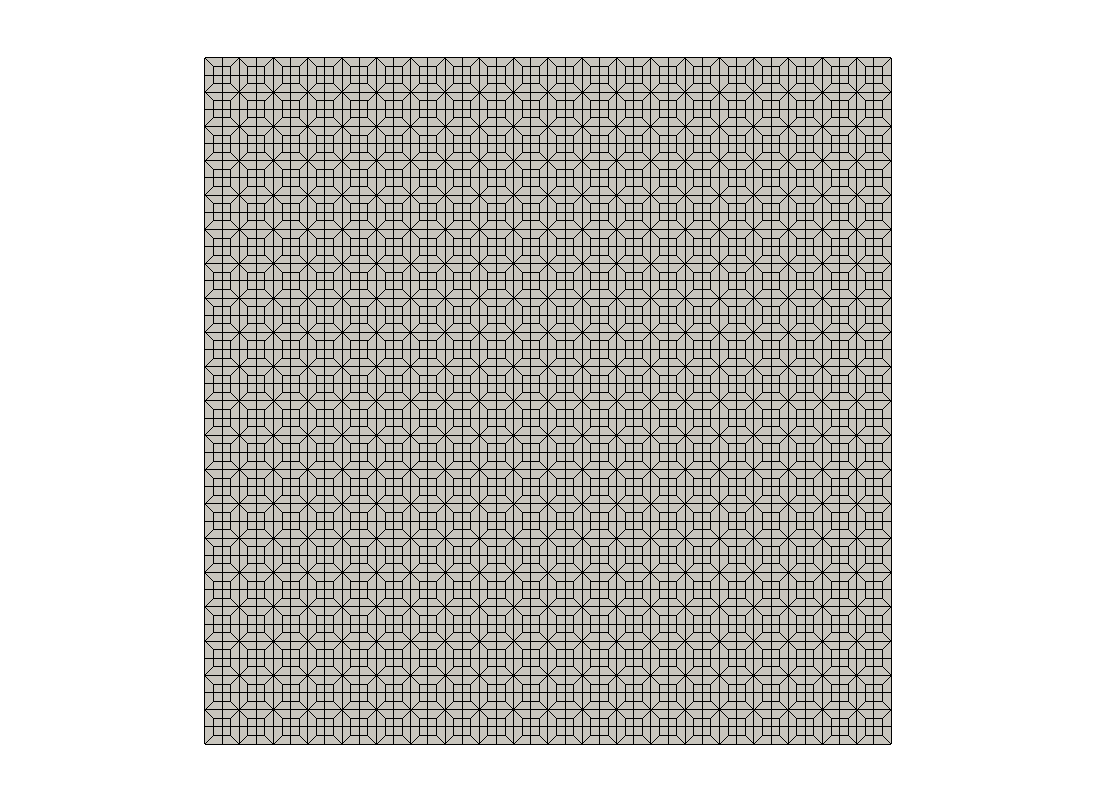
\includegraphics[width=7cm]{python_codes/fieldstone_78/results/mms/grid2}
d)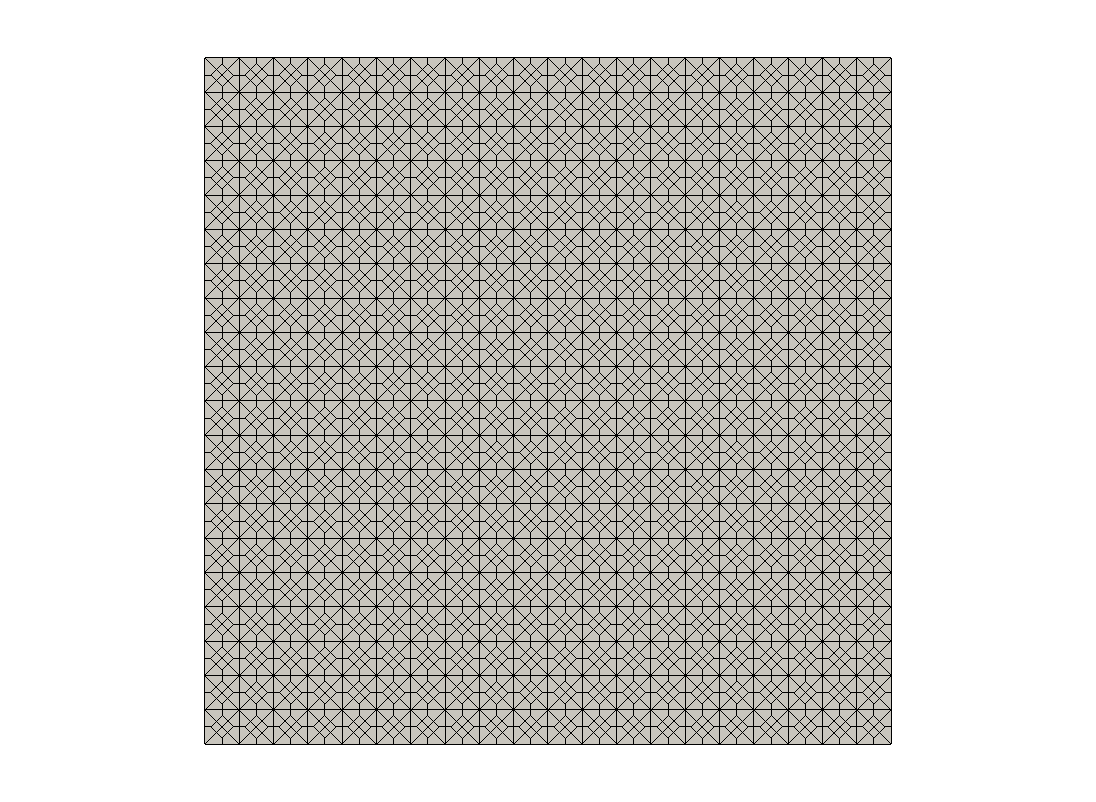
\includegraphics[width=7cm]{python_codes/fieldstone_78/results/mms/grid3}\\
{\captionfont Meshes composed of 4800 elements. a) regular; b) Stenberg macro-elementl 
c) Le Tallec macro-element; d) Qin \& Zhang macro-element.}
\end{center}

Pressure normalisation is achieved by setting $p=0$ on the last element and then 
renormalising the pressure field so that $\int p dV=0$.

%........................
\paragraph{Results - mms}

We start with the Donea \& Huerta manufactured solution (see Section~\ref{mms1}) and 
proceed to compute the velocity and pressure error convergence as a function of the 
element size which is taken to be $h = \sqrt{L_xL_y/nel}$. We see that 
the errors converge as expected, quadratically for the velocity and linearly for the pressure.
Rather interestingly the projection of the pressure onto the nodes has a convergence rate 
higher than the raw elemental pressure. As predicted in Qin \& Zhang, the Stenberg macro-element 
yields the best results, followed by the Le Tallec and then the one they propose (this conclusion 
is logically supported by looking at root mean square velocity measurements). 
Finally, the presence of the checkerboard makes it painfully clear that it is the worst element 
and the pressure error does not converge.  

\begin{center}
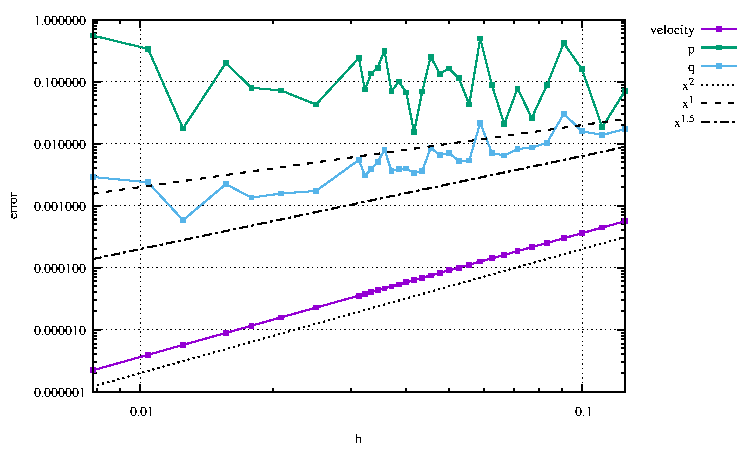
\includegraphics[width=7cm]{python_codes/fieldstone_78/results/mms/errors_regular.pdf}
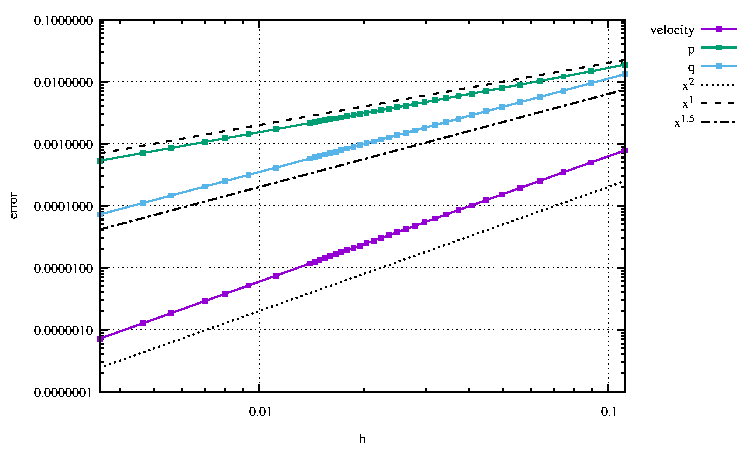
\includegraphics[width=7cm]{python_codes/fieldstone_78/results/mms/errors_stenberg.pdf}\\
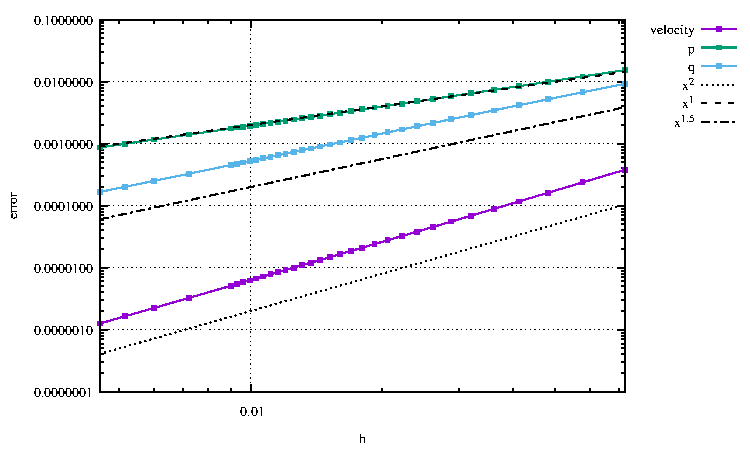
\includegraphics[width=7cm]{python_codes/fieldstone_78/results/mms/errors_letallec.pdf}
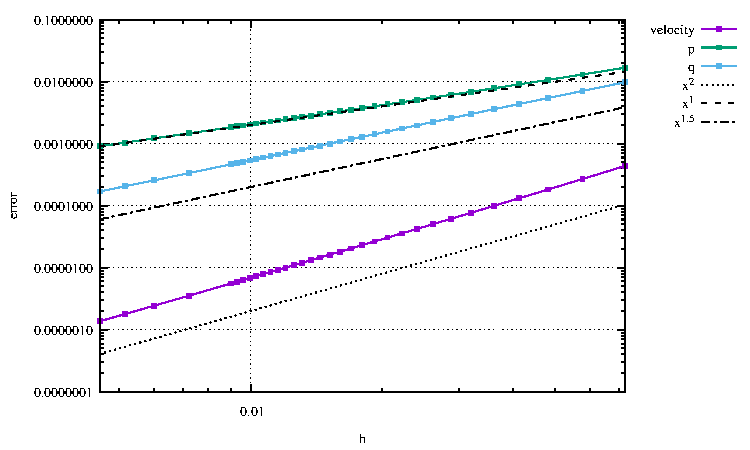
\includegraphics[width=7cm]{python_codes/fieldstone_78/results/mms/errors_qinzhang.pdf}\\
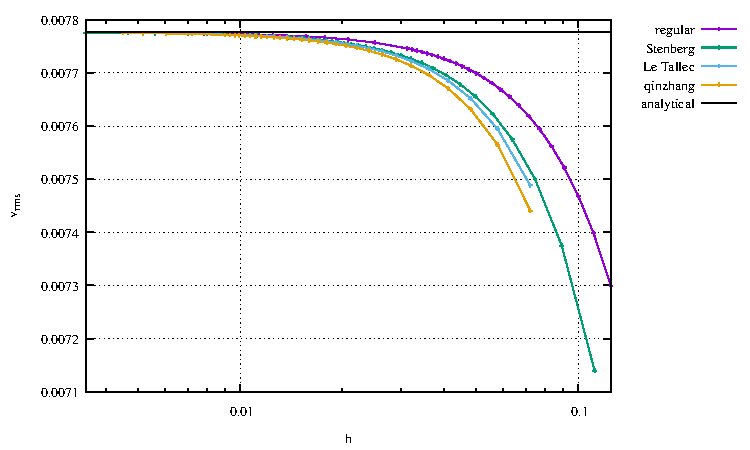
\includegraphics[width=8cm]{python_codes/fieldstone_78/results/mms/vrms.pdf}
\end{center}

On the following figures the pressure is plotted against the analytical solution and 
we see that there is no checkerboarding occurring:
Rather interestingly the pressure error is the largest next to the boundaries:

\begin{center}
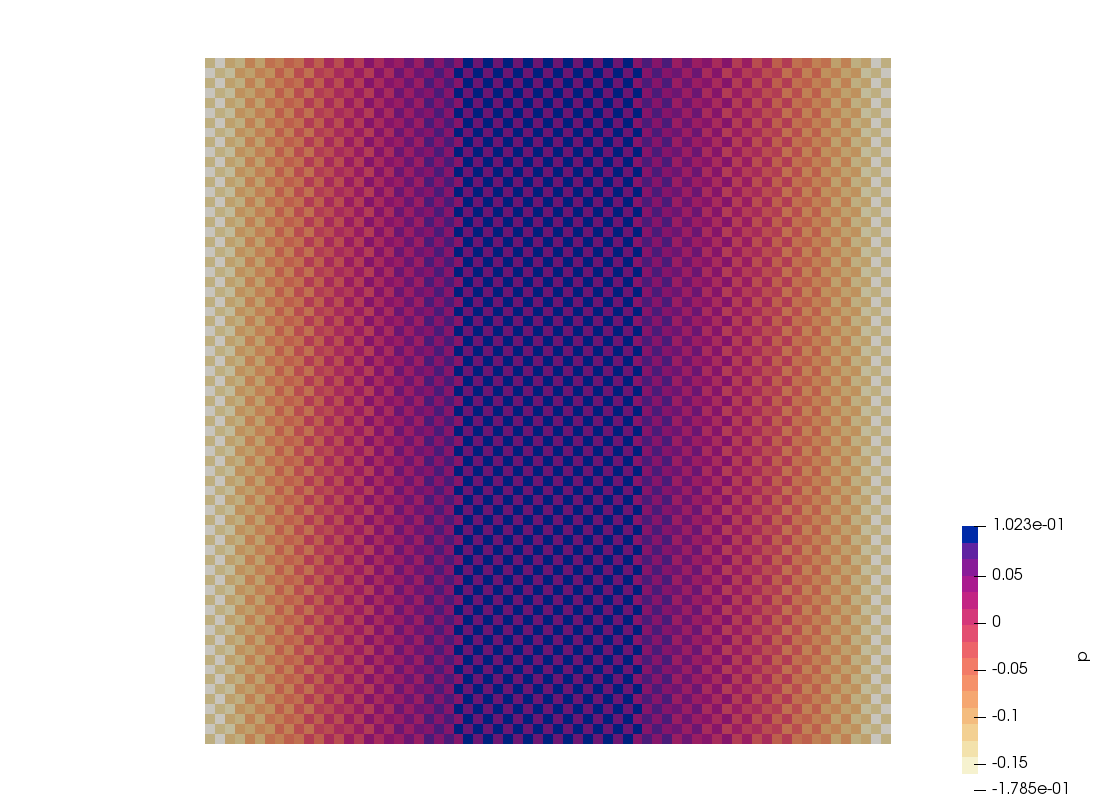
\includegraphics[width=3.74cm]{python_codes/fieldstone_78/results/mms/p_0}
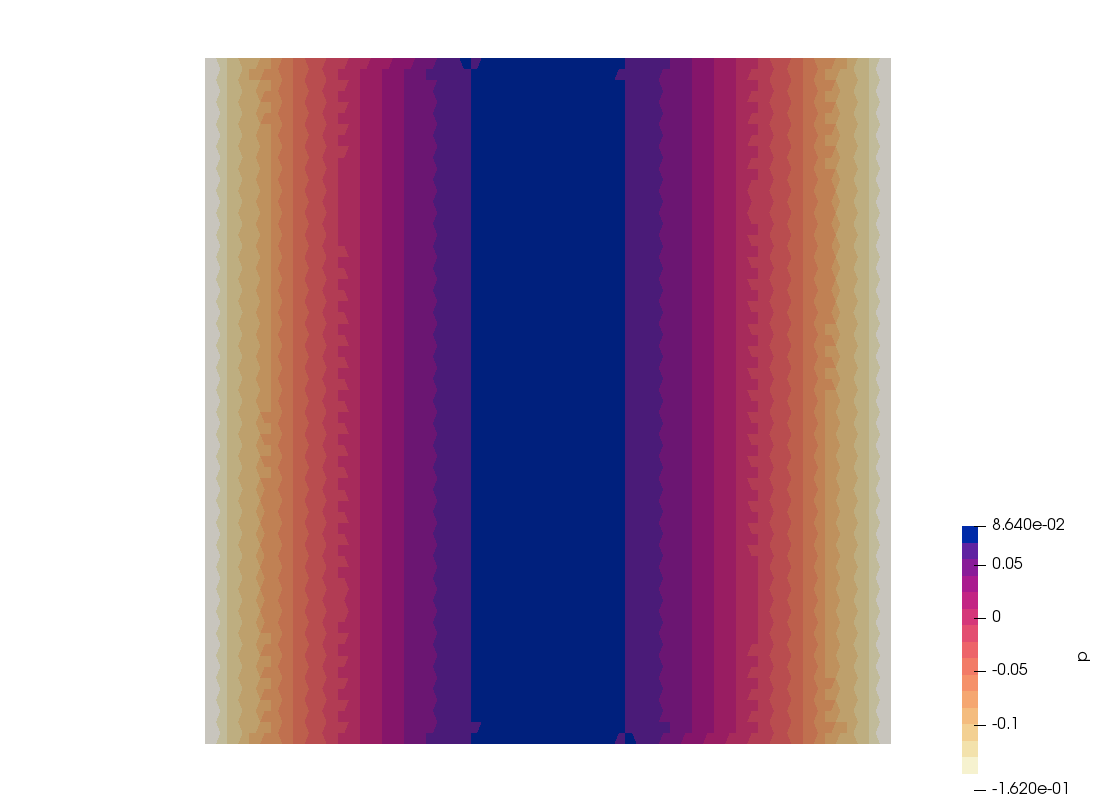
\includegraphics[width=3.74cm]{python_codes/fieldstone_78/results/mms/p_1}
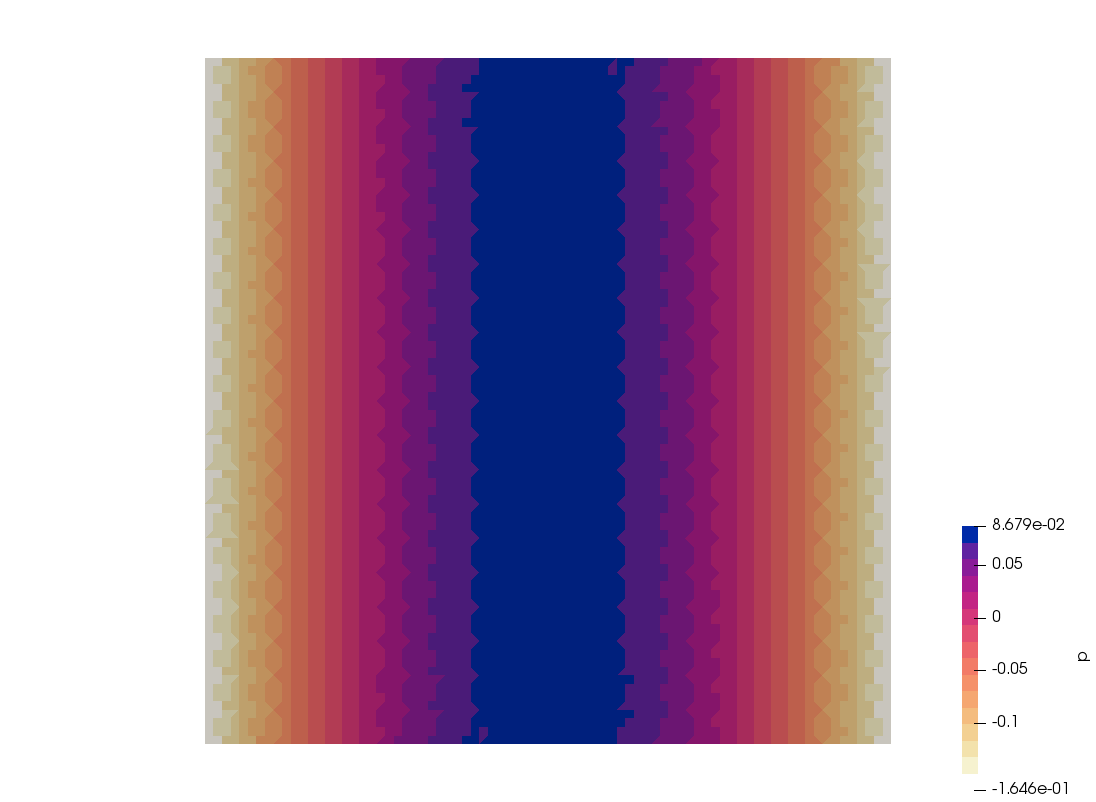
\includegraphics[width=3.74cm]{python_codes/fieldstone_78/results/mms/p_2}
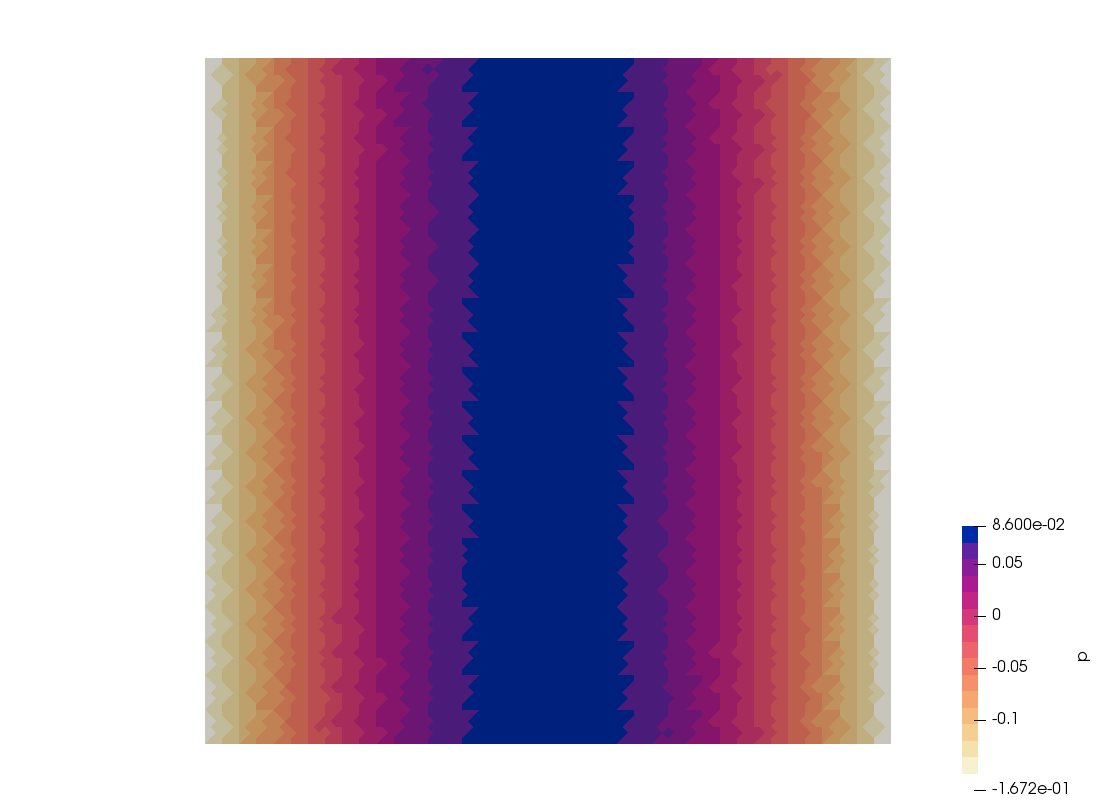
\includegraphics[width=3.74cm]{python_codes/fieldstone_78/results/mms/p_3}\\
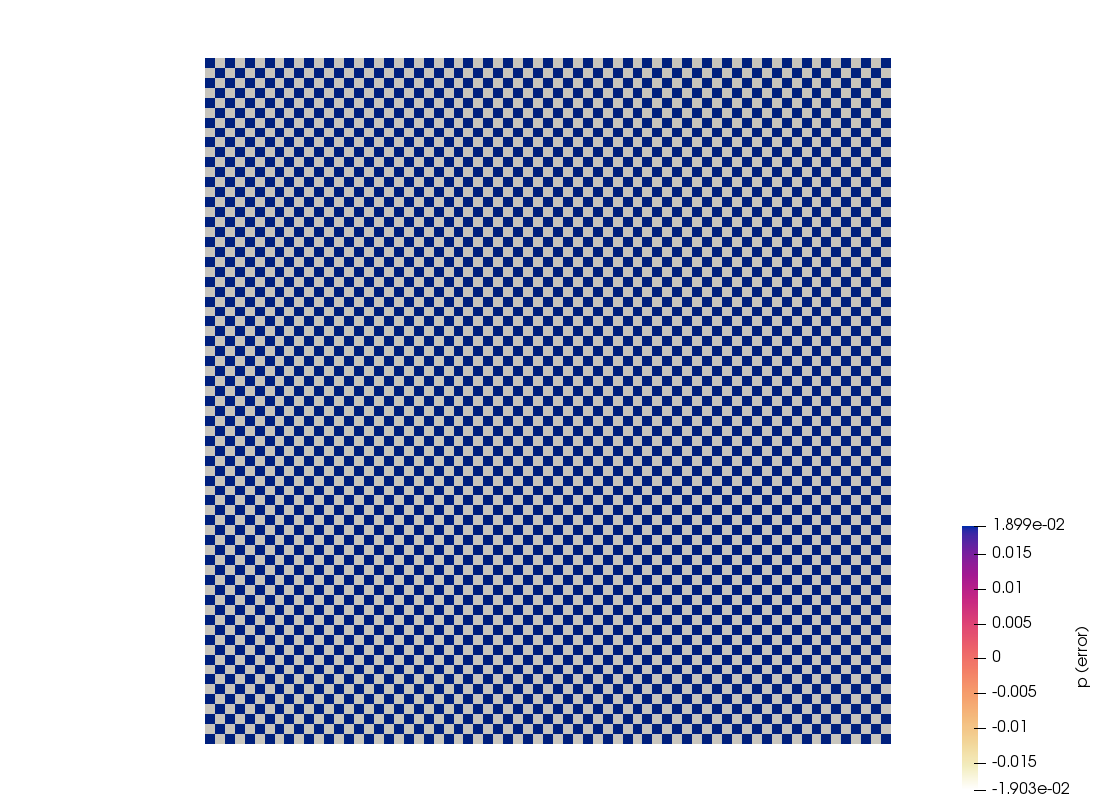
\includegraphics[width=3.74cm]{python_codes/fieldstone_78/results/mms/p_error_0}
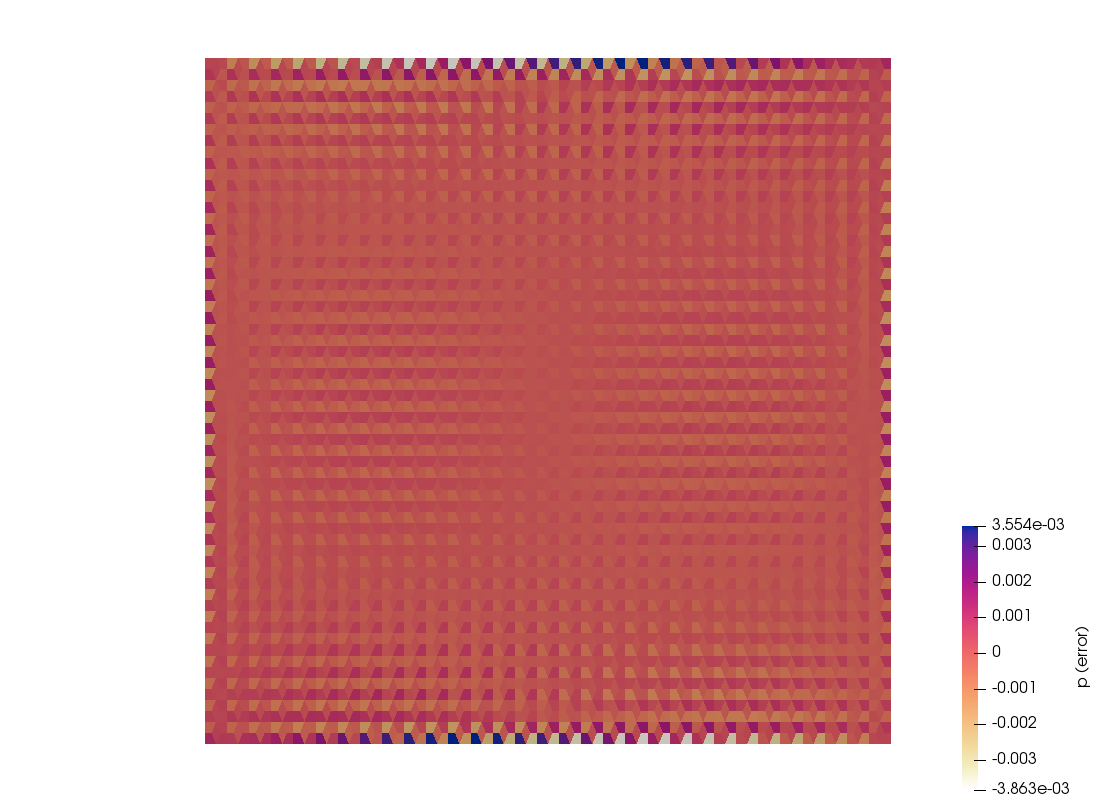
\includegraphics[width=3.74cm]{python_codes/fieldstone_78/results/mms/p_error_1}
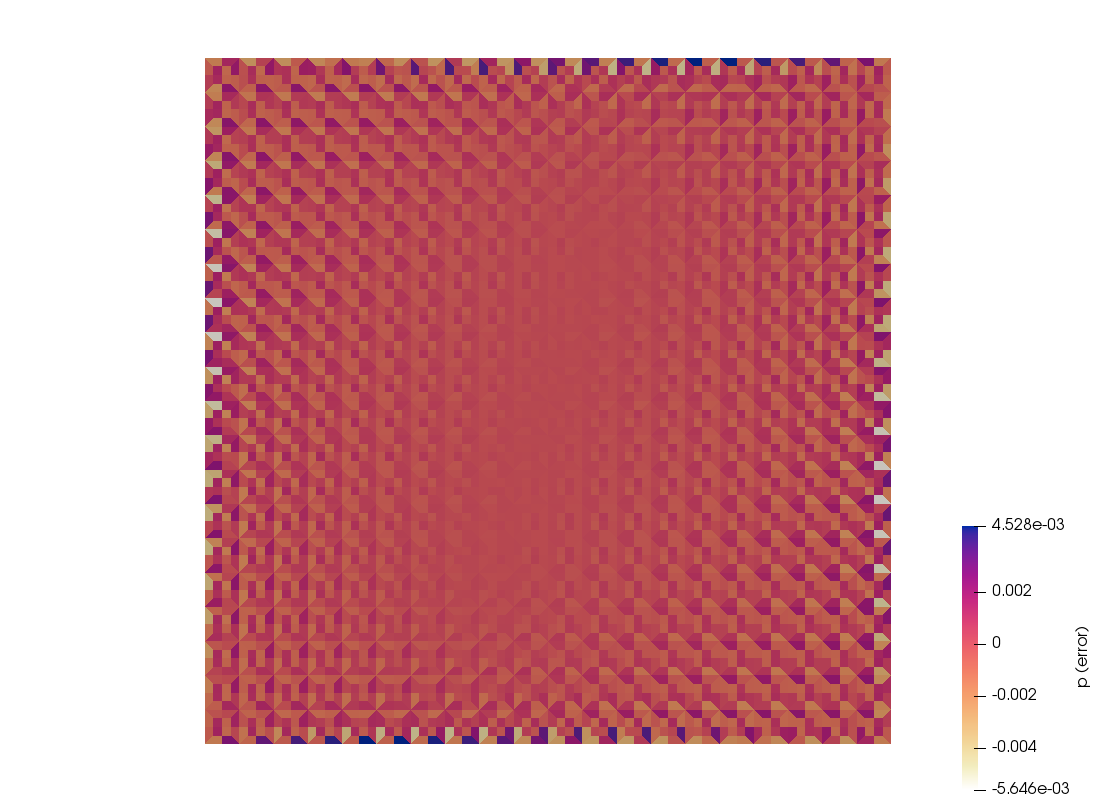
\includegraphics[width=3.74cm]{python_codes/fieldstone_78/results/mms/p_error_2}
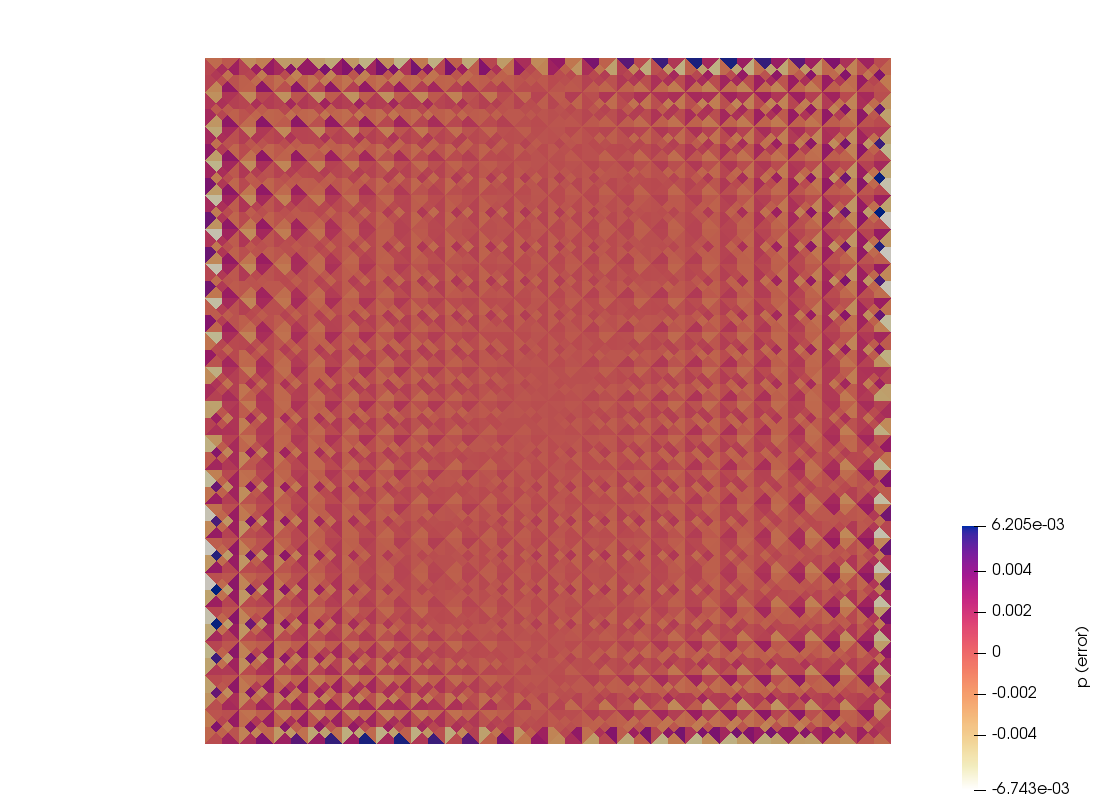
\includegraphics[width=3.74cm]{python_codes/fieldstone_78/results/mms/p_error_3}\\
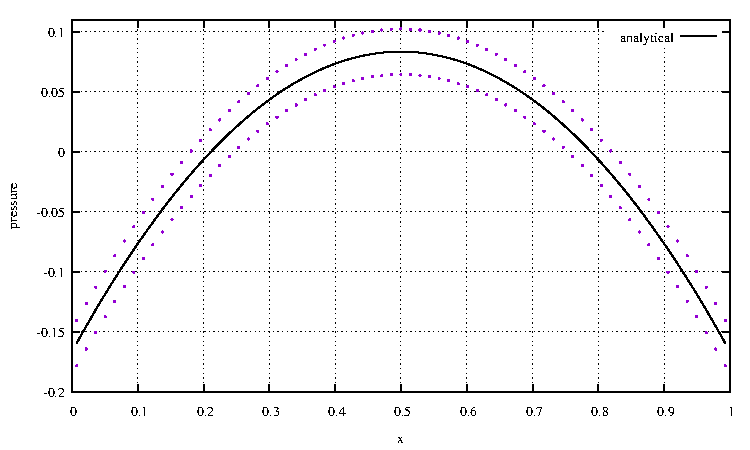
\includegraphics[width=3.74cm]{python_codes/fieldstone_78/results/mms/pressure0}
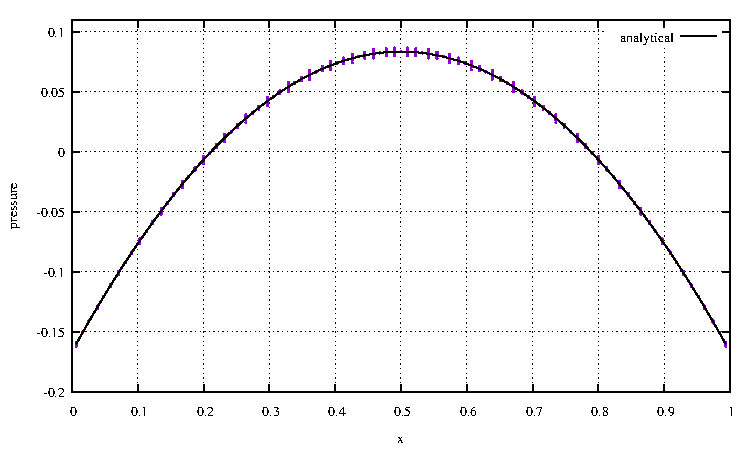
\includegraphics[width=3.74cm]{python_codes/fieldstone_78/results/mms/pressure1}
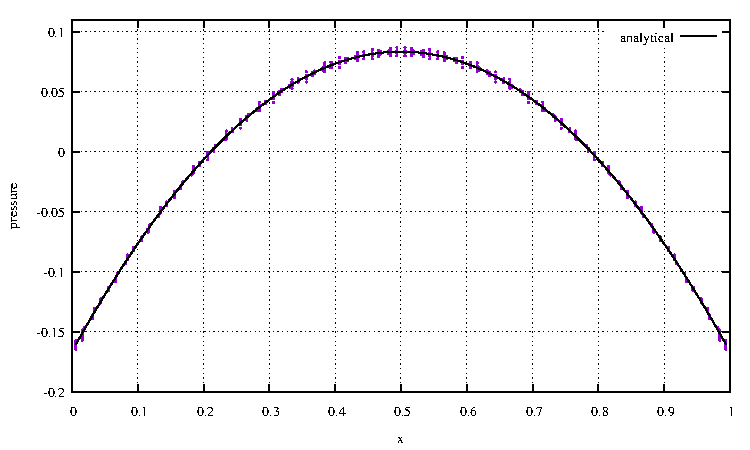
\includegraphics[width=3.74cm]{python_codes/fieldstone_78/results/mms/pressure2}
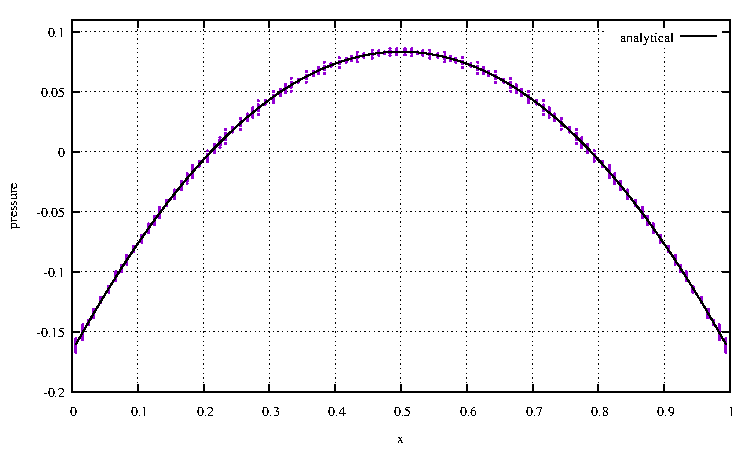
\includegraphics[width=3.74cm]{python_codes/fieldstone_78/results/mms/pressure3}\\
{\captionfont Meshes count about the same number of elements, i.e. 4800. 
Left to right: regular, Stenberg, Le Tallec, Qin \& Zhang. Top row is pressure, 
middle row is pressure error. Bottom row is pressure profile.} 
\end{center}



Discussion: what is the real advantage of such a macro-element? it is LBB stable, so 
iterative solver will work optimally, and the pressure has no checkerboard. 
Also the number of non-zeros per line of the matrix is small.  
On the other hand it is anisotropic since the 'diamonds are vertical'. 
Also if one would consider a macro-element as an element, it counts 10 velocity nodes and 5 pressures, 
which makes it much more expensive than a $Q_2\times Q_1$ element of the same size...






\newpage
%..................................
\paragraph{Results - Aquarium}

\begin{center}
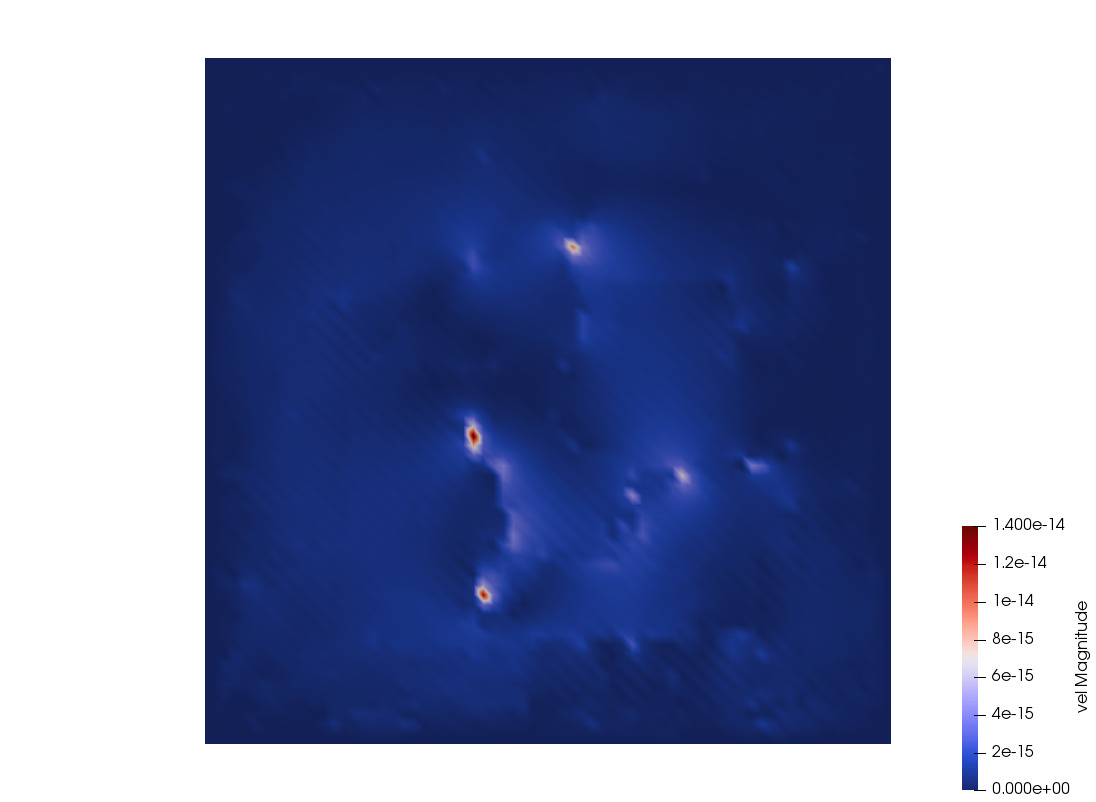
\includegraphics[width=3.8cm]{python_codes/fieldstone_78/results/aquarium/vel0}
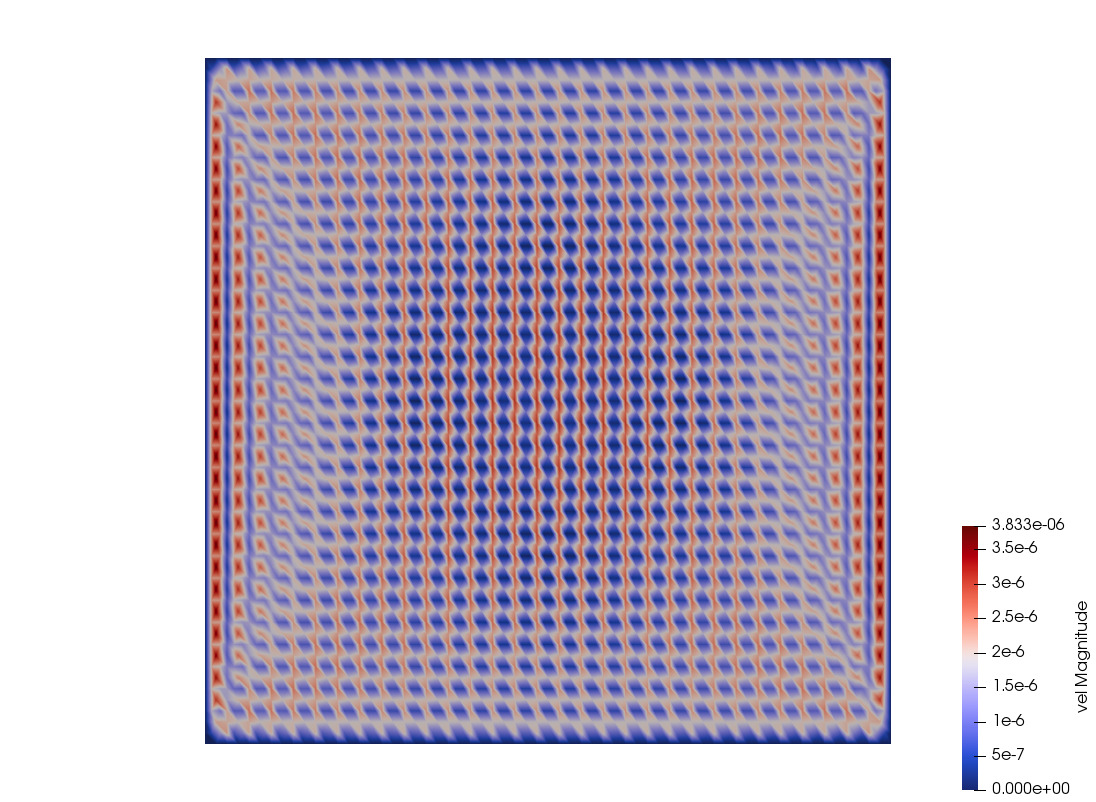
\includegraphics[width=3.8cm]{python_codes/fieldstone_78/results/aquarium/vel1}
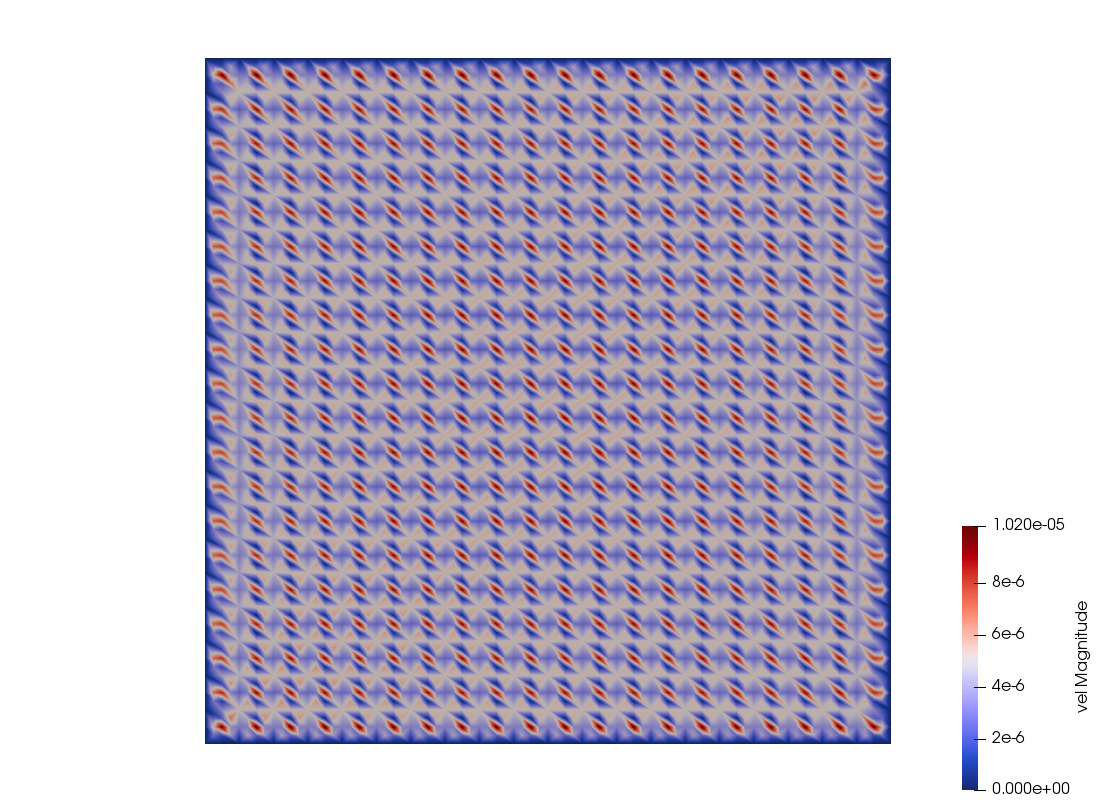
\includegraphics[width=3.8cm]{python_codes/fieldstone_78/results/aquarium/vel2}
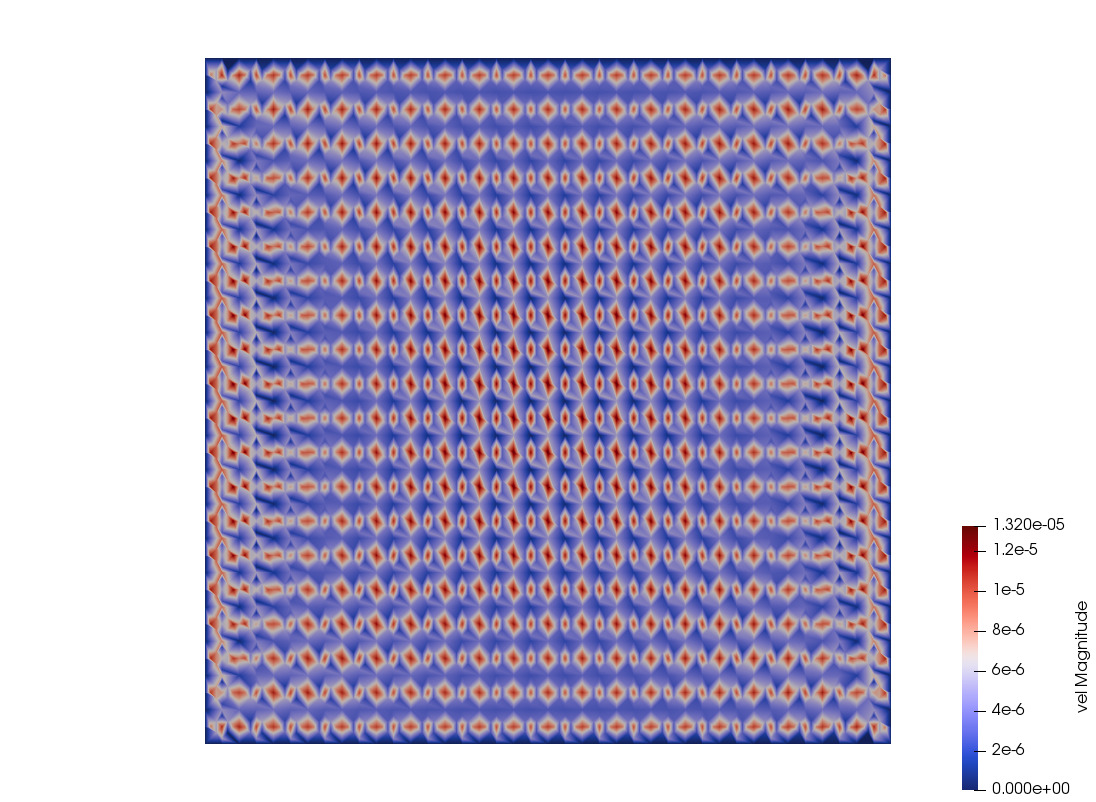
\includegraphics[width=3.8cm]{python_codes/fieldstone_78/results/aquarium/vel3}\\
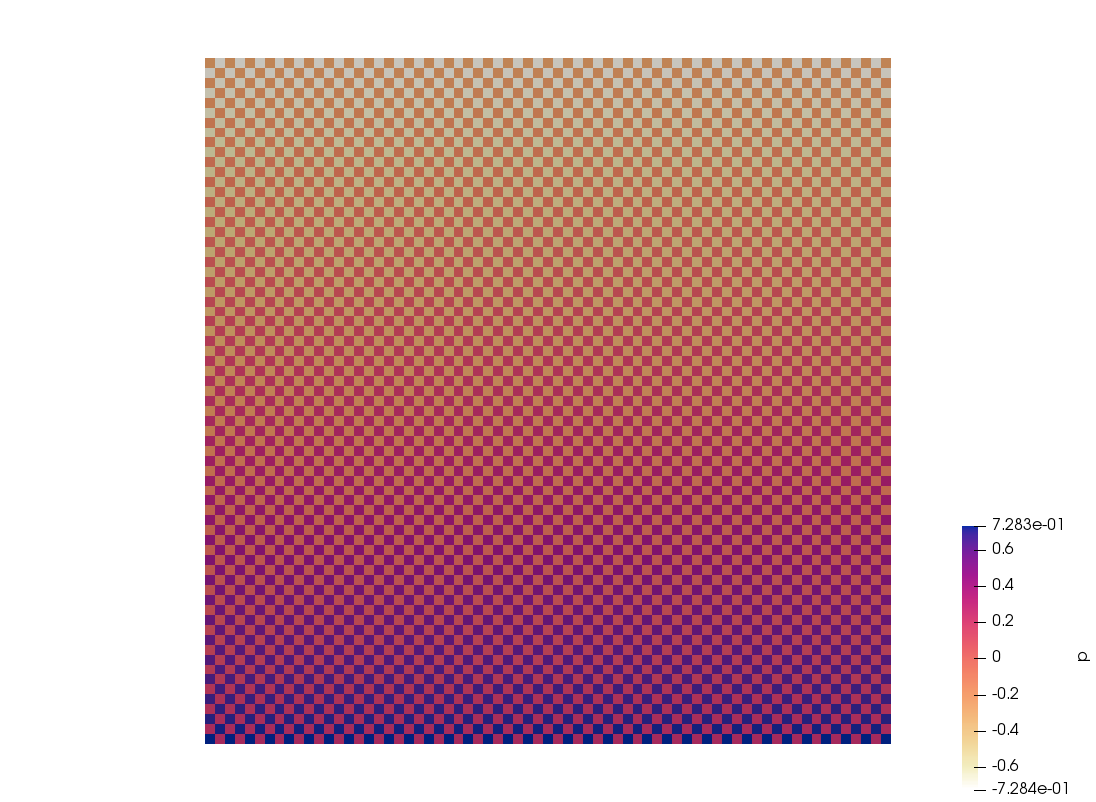
\includegraphics[width=3.8cm]{python_codes/fieldstone_78/results/aquarium/p0}
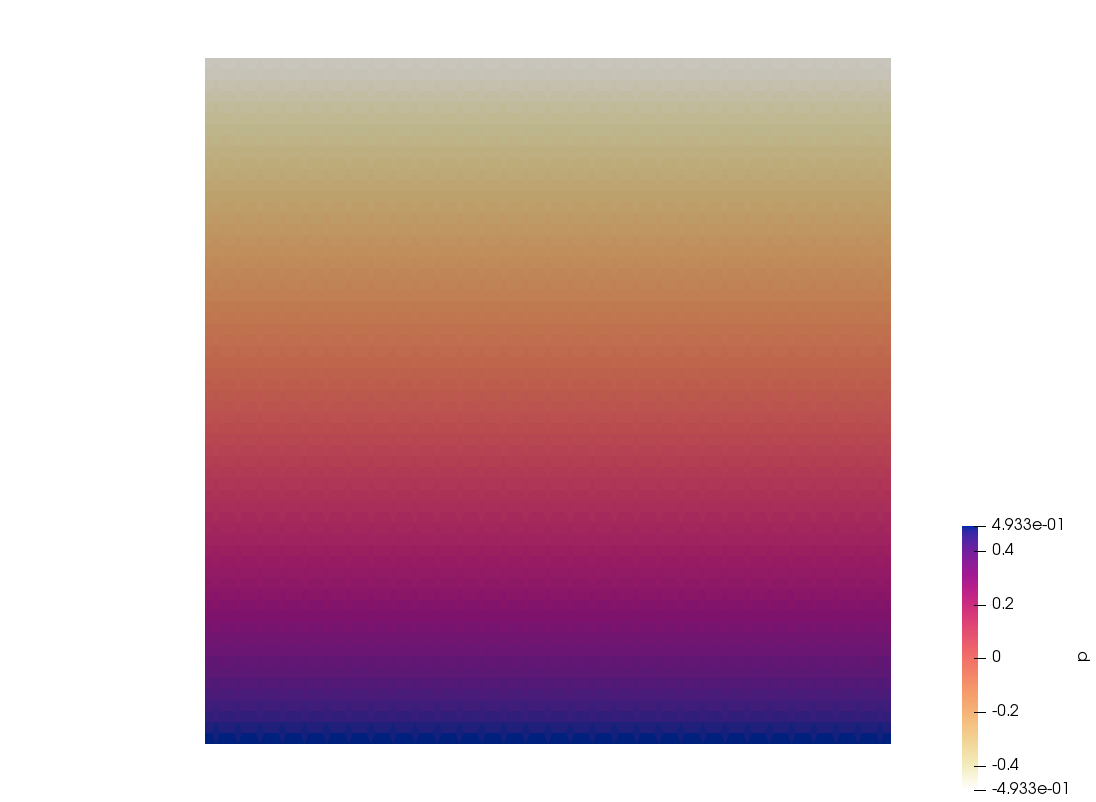
\includegraphics[width=3.8cm]{python_codes/fieldstone_78/results/aquarium/p1}
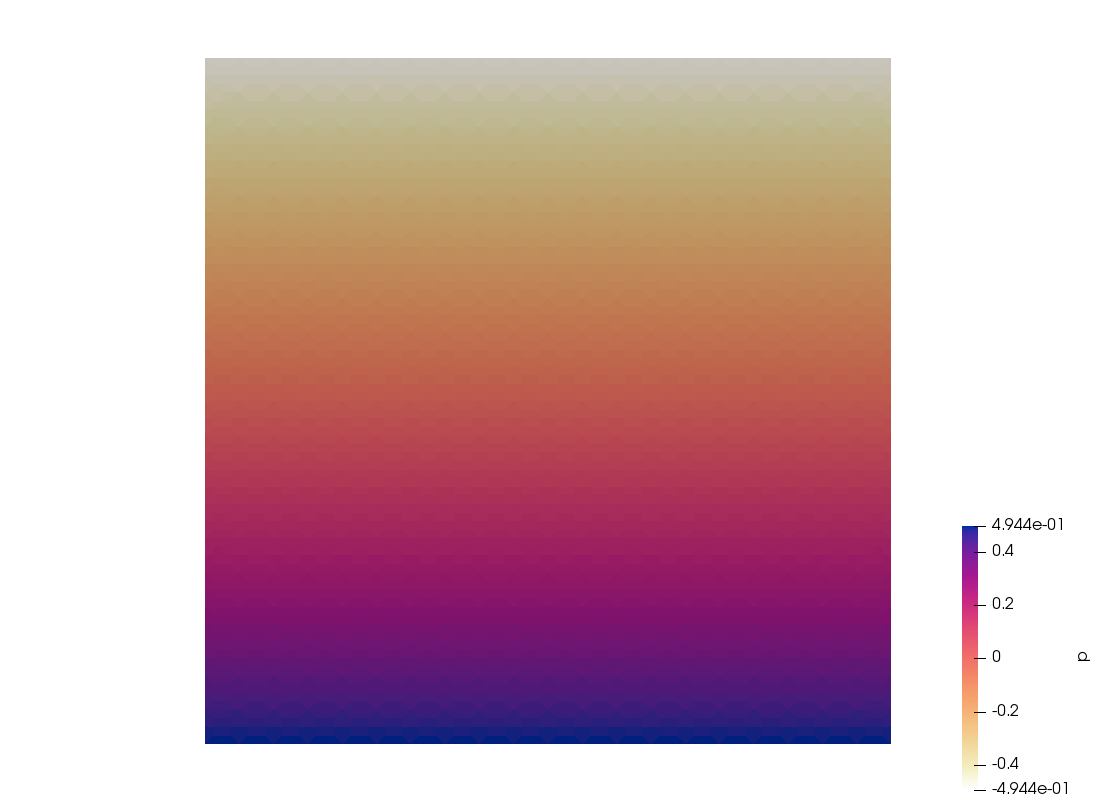
\includegraphics[width=3.8cm]{python_codes/fieldstone_78/results/aquarium/p2}
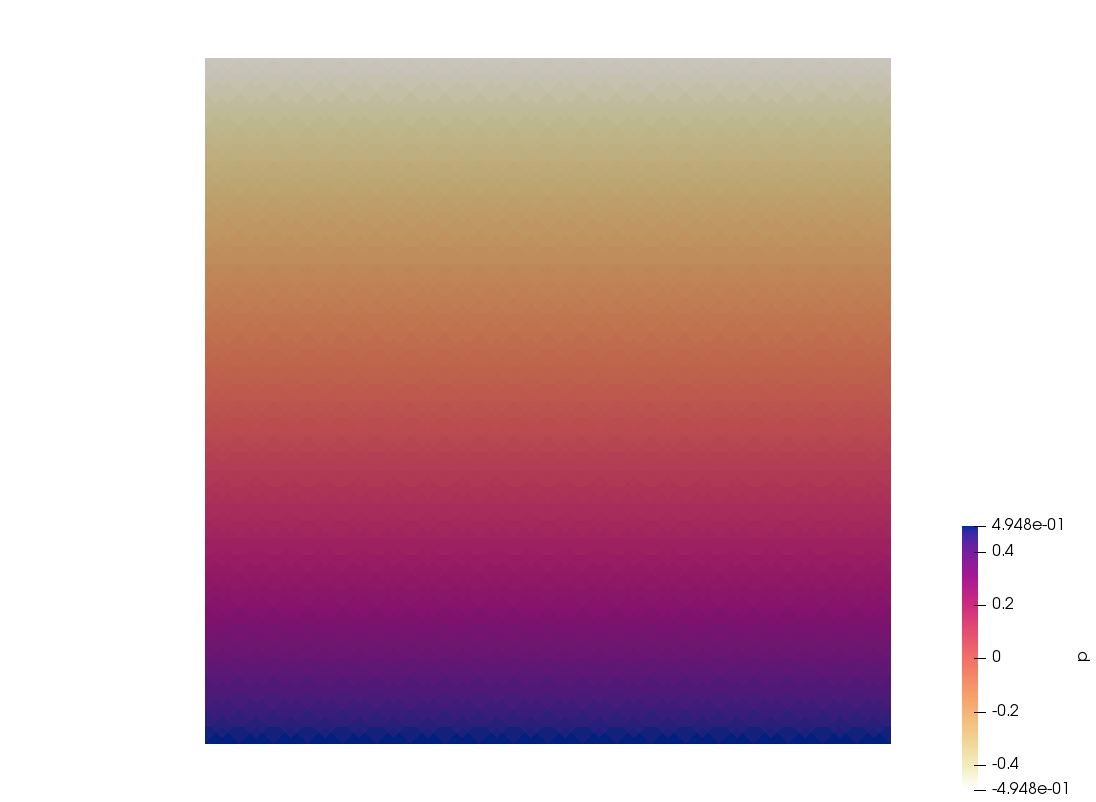
\includegraphics[width=3.8cm]{python_codes/fieldstone_78/results/aquarium/p3}\\
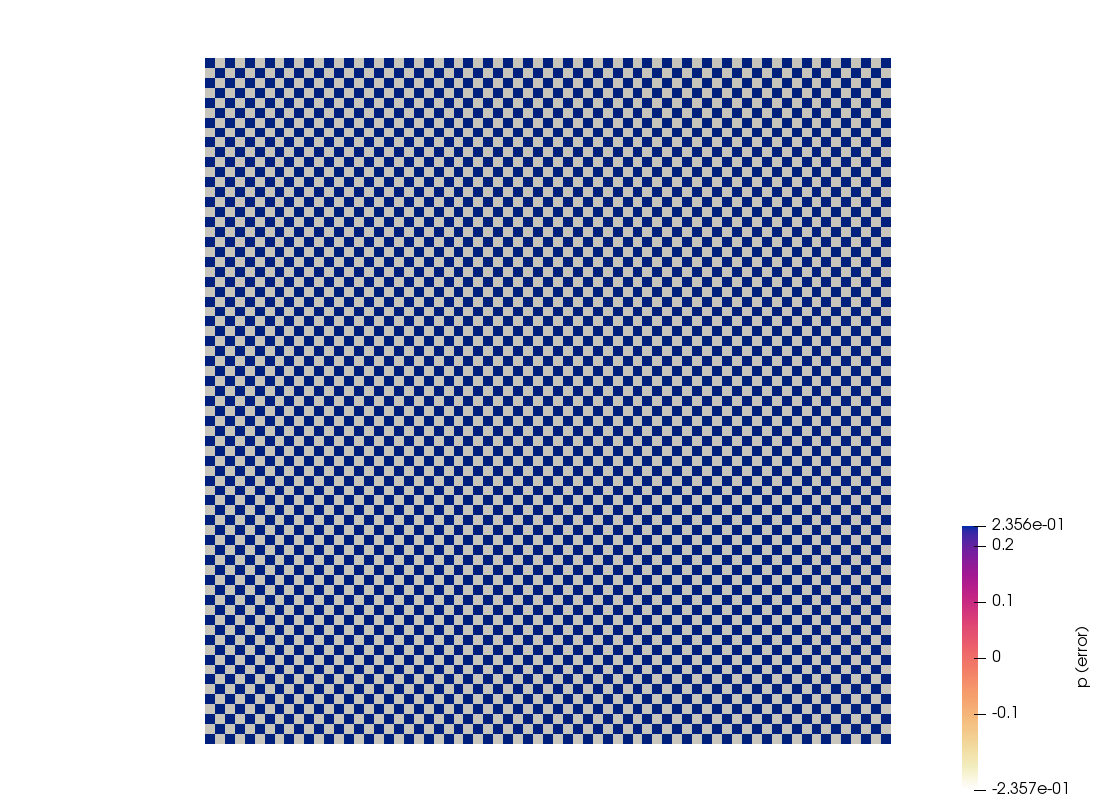
\includegraphics[width=3.8cm]{python_codes/fieldstone_78/results/aquarium/p_error_0}
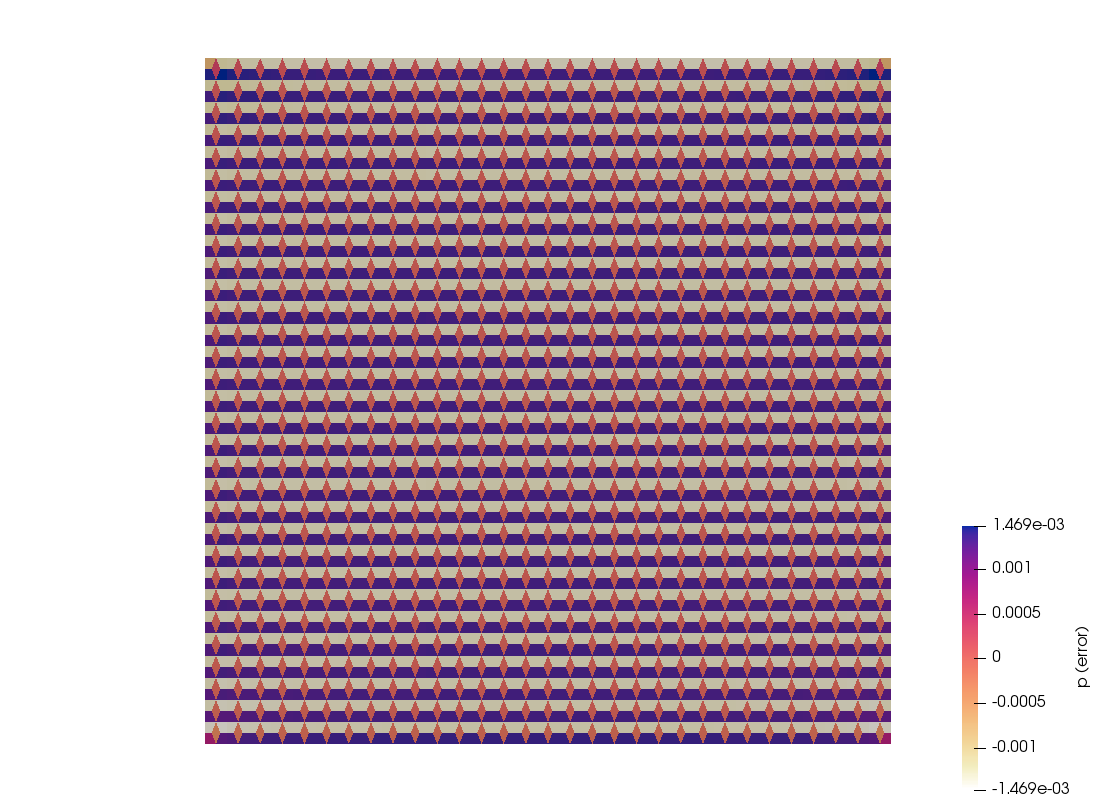
\includegraphics[width=3.8cm]{python_codes/fieldstone_78/results/aquarium/p_error_1}
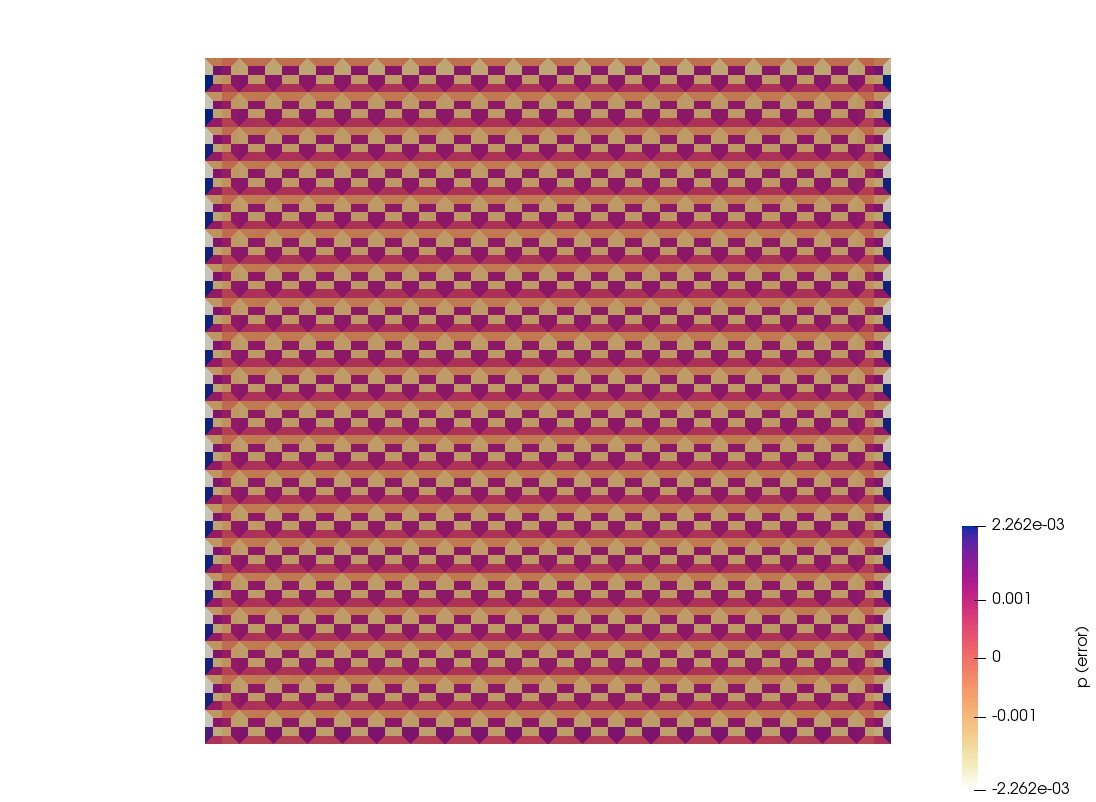
\includegraphics[width=3.8cm]{python_codes/fieldstone_78/results/aquarium/p_error_2}
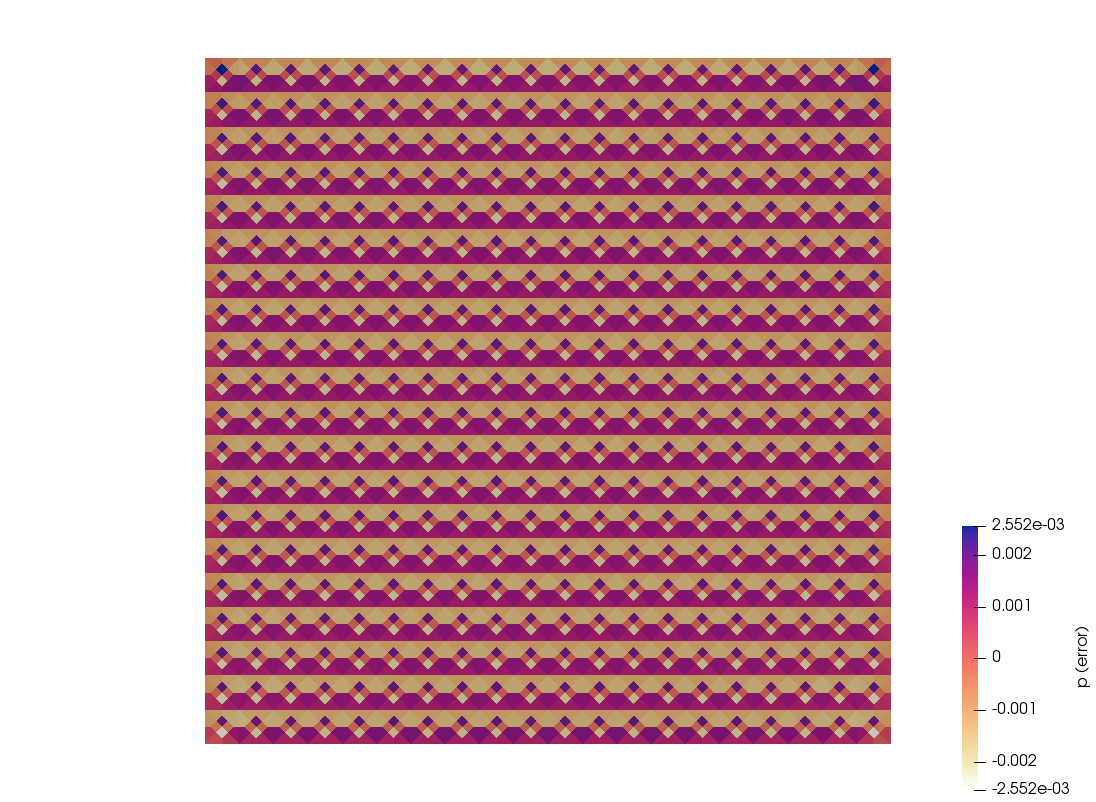
\includegraphics[width=3.8cm]{python_codes/fieldstone_78/results/aquarium/p_error_3}\\
{\captionfont velocity, pressure and pressure error 
fields for regular, Stenberg, Le Tallec, Qin \& Zhang.} 
\end{center}

\begin{center}
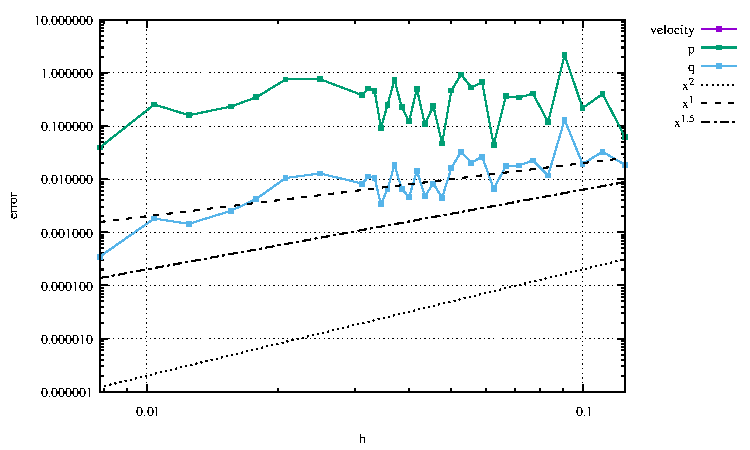
\includegraphics[width=3.74cm]{python_codes/fieldstone_78/results/aquarium/errors_regular.pdf}
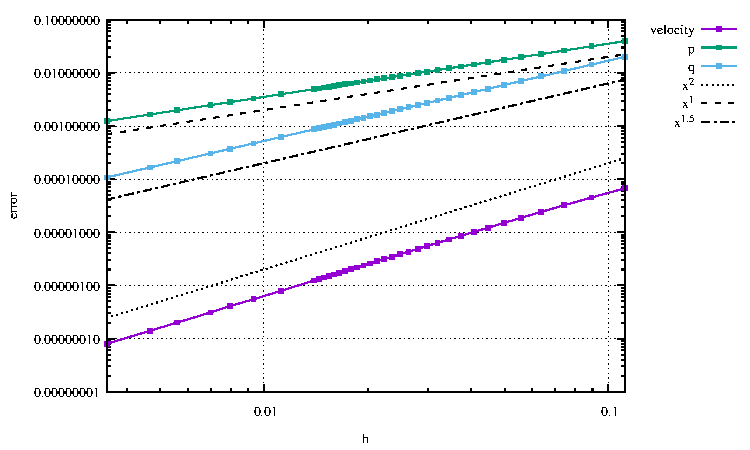
\includegraphics[width=3.74cm]{python_codes/fieldstone_78/results/aquarium/errors_stenberg.pdf}
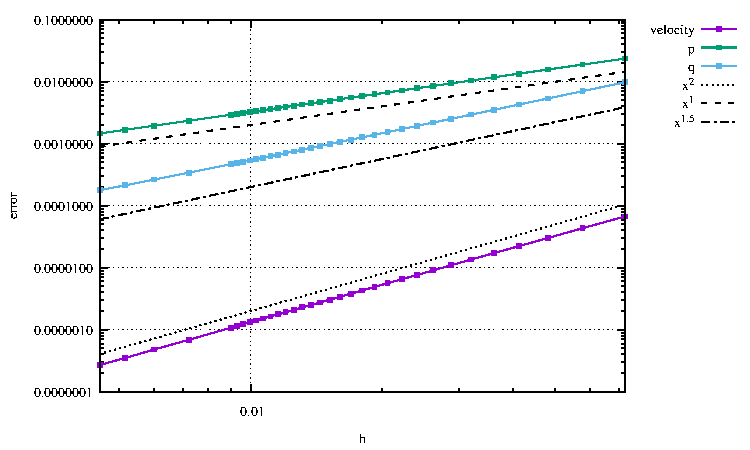
\includegraphics[width=3.74cm]{python_codes/fieldstone_78/results/aquarium/errors_letallec.pdf}
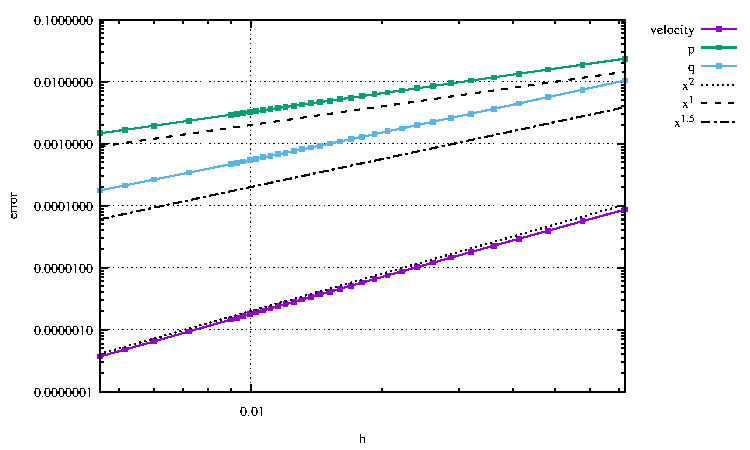
\includegraphics[width=3.74cm]{python_codes/fieldstone_78/results/aquarium/errors_qinzhang.pdf}\\
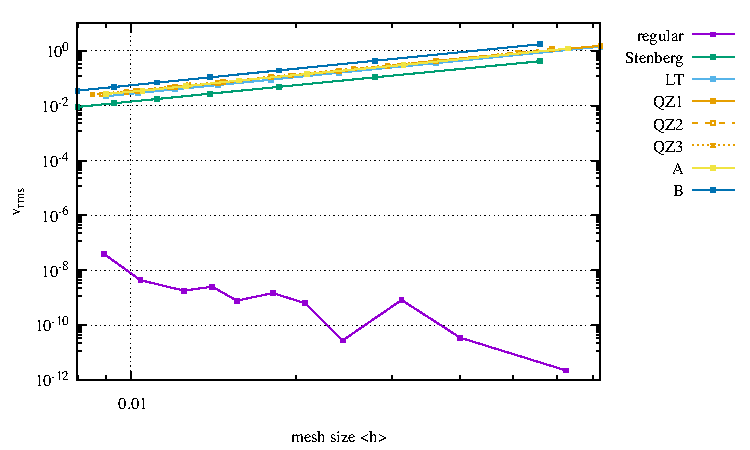
\includegraphics[width=8cm]{python_codes/fieldstone_78/results/aquarium/vrms.pdf}
\end{center}



Stenberg is better: lower velocity error and pressure error.


\newpage
%.....................................................
\paragraph{Results - sinking block - reduced density}

The block has size 0.25x0.25, centered in the domain. No-slip boundary conditions are imposed on all 
sides. The buoyancy force $\rho g_y$ is -1 in the block and zero elsewhere. Viscosity is constant and 
equal to 1 everywhere. 

\begin{center}
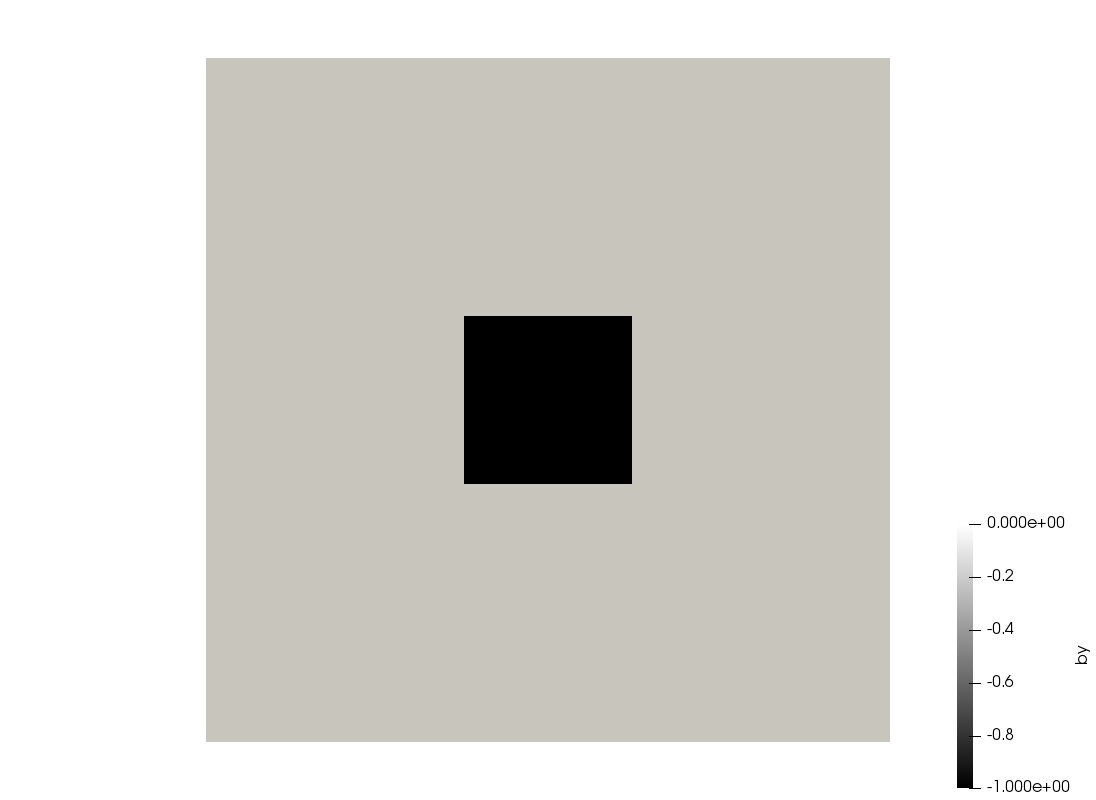
\includegraphics[width=3.8cm]{python_codes/fieldstone_78/results/block/reduced/by0}
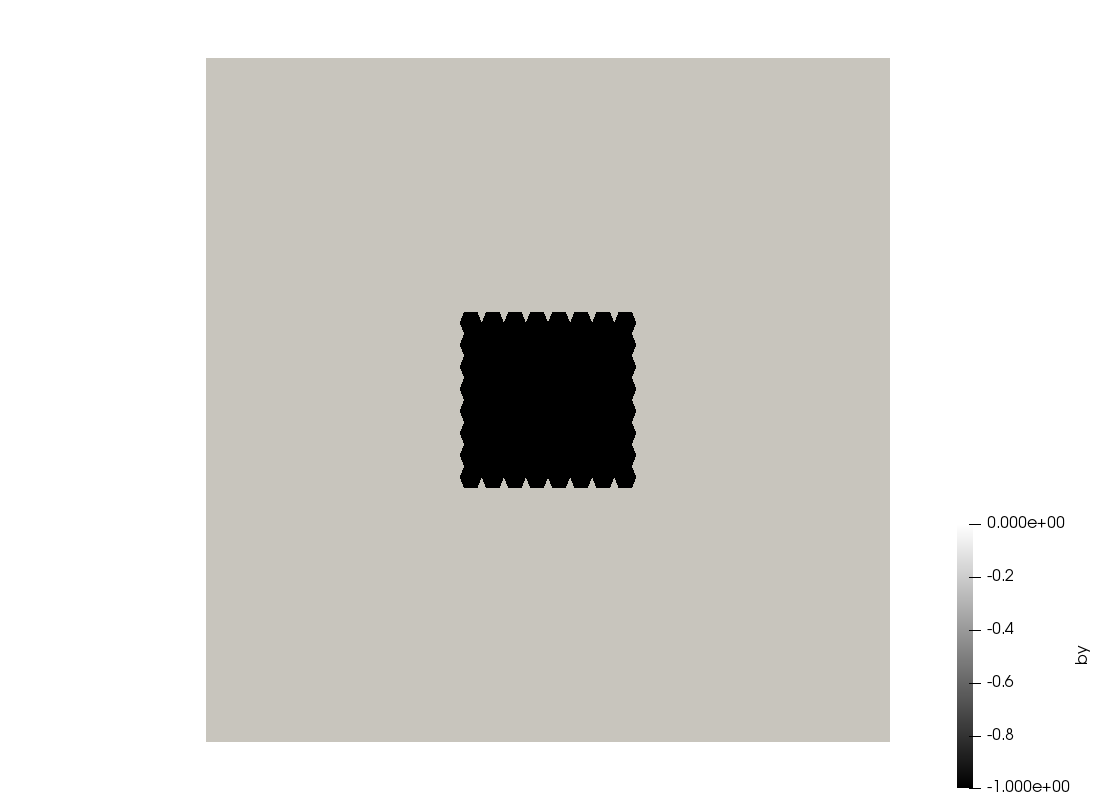
\includegraphics[width=3.8cm]{python_codes/fieldstone_78/results/block/reduced/by1}
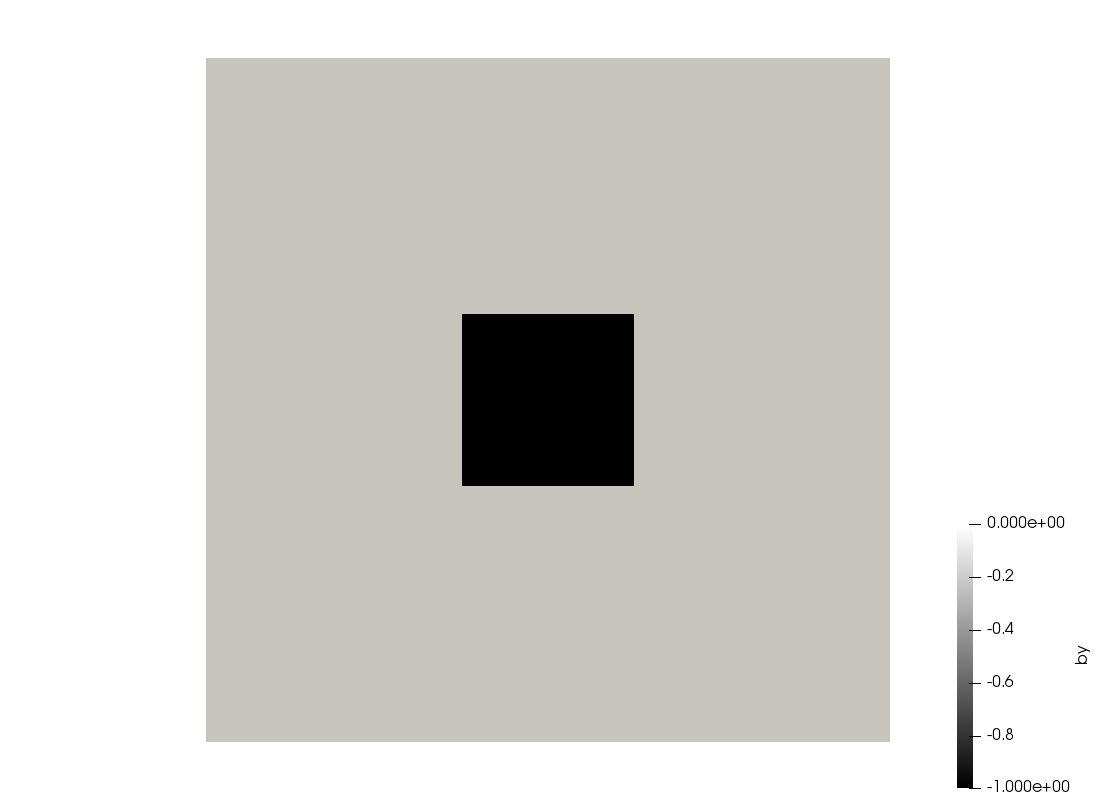
\includegraphics[width=3.8cm]{python_codes/fieldstone_78/results/block/reduced/by2}
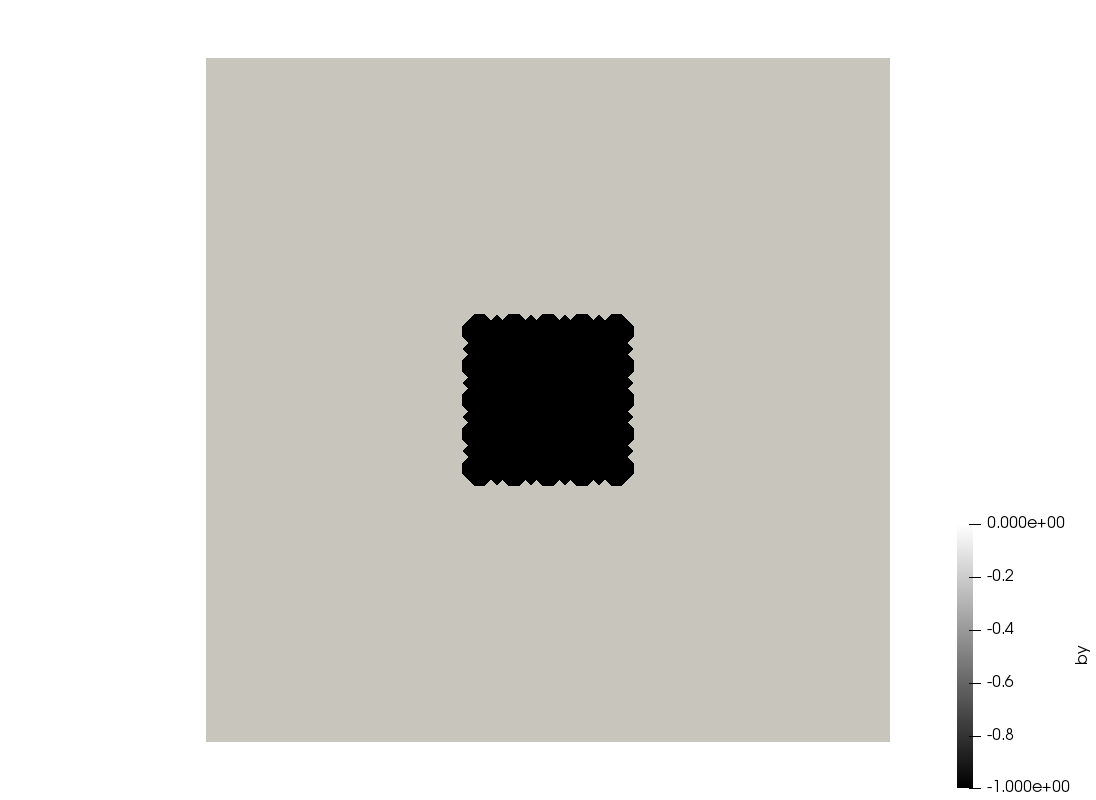
\includegraphics[width=3.8cm]{python_codes/fieldstone_78/results/block/reduced/by3}\\
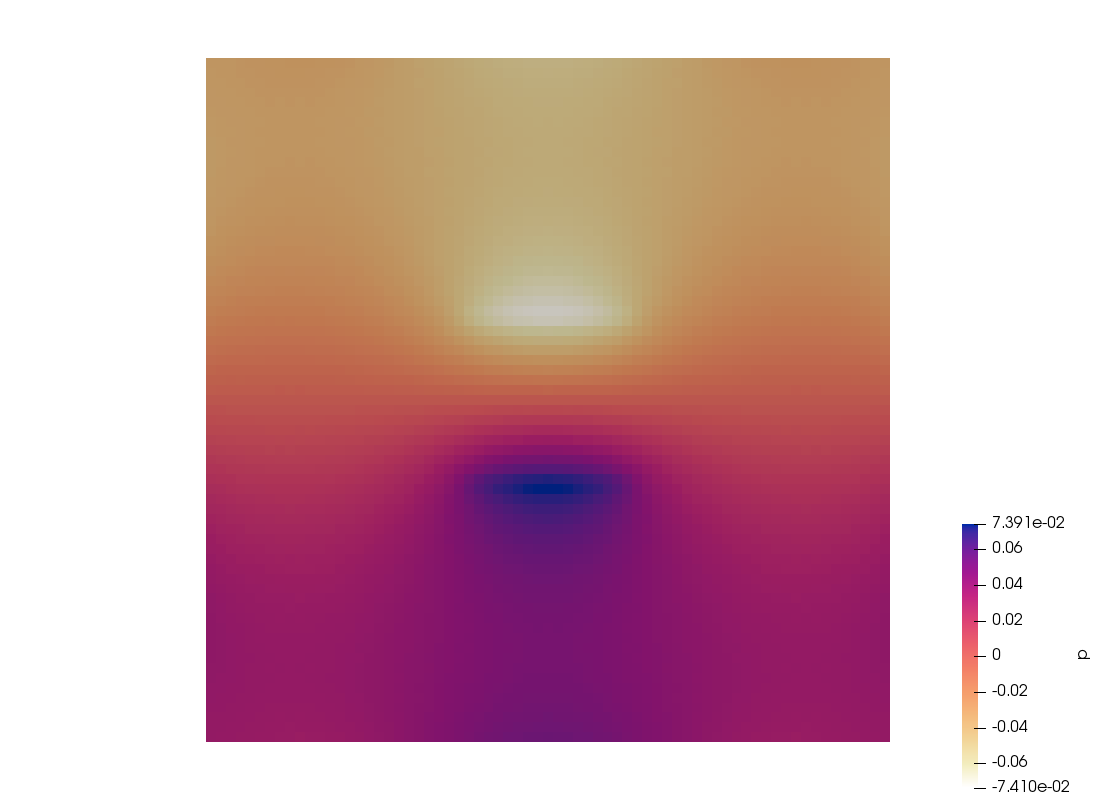
\includegraphics[width=3.8cm]{python_codes/fieldstone_78/results/block/reduced/p0}
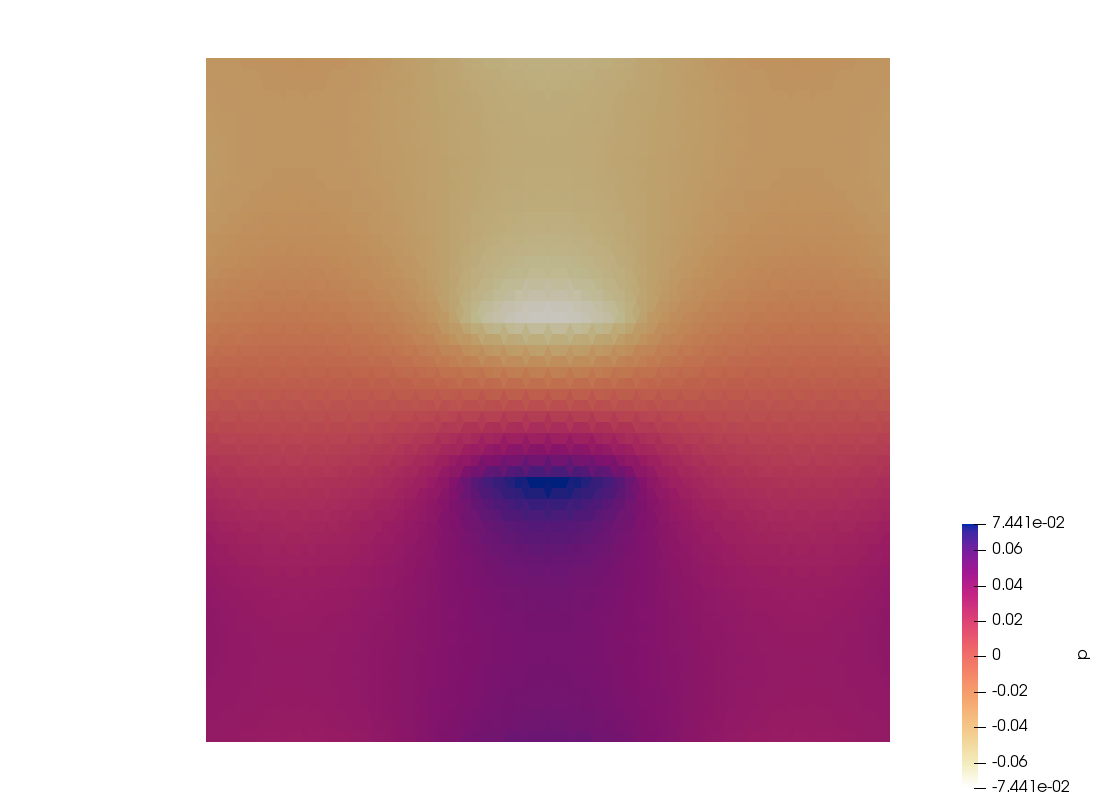
\includegraphics[width=3.8cm]{python_codes/fieldstone_78/results/block/reduced/p1}
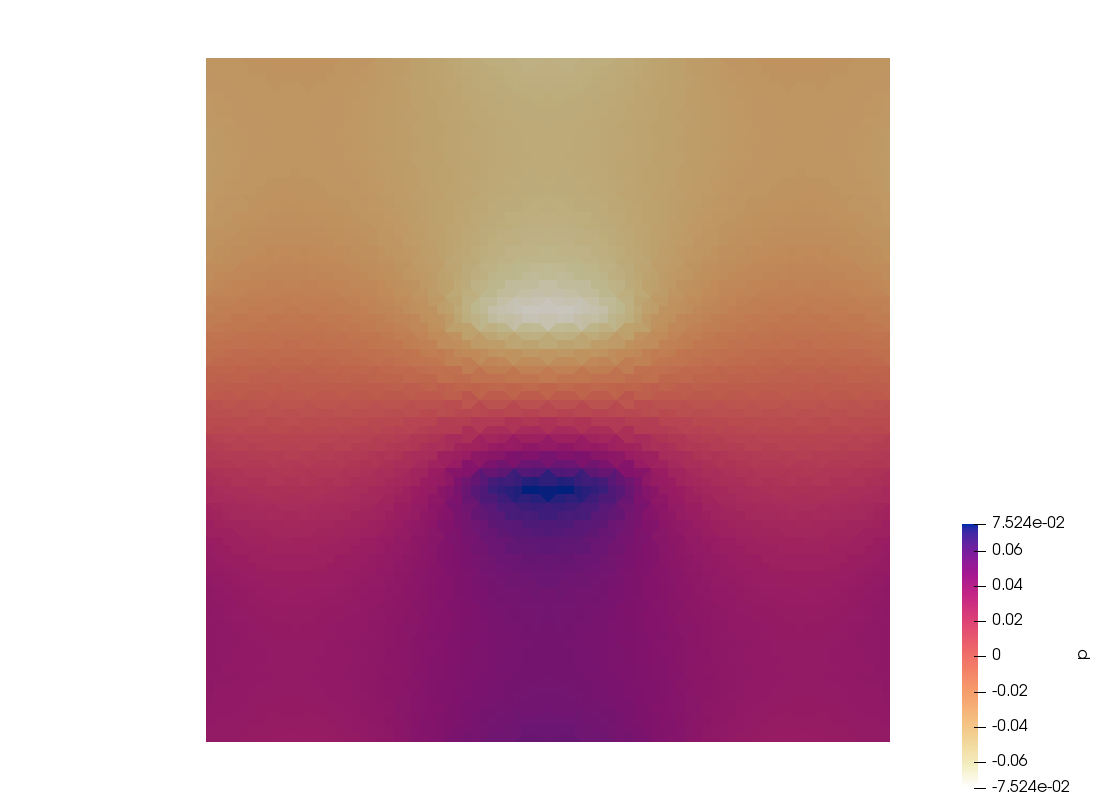
\includegraphics[width=3.8cm]{python_codes/fieldstone_78/results/block/reduced/p2}
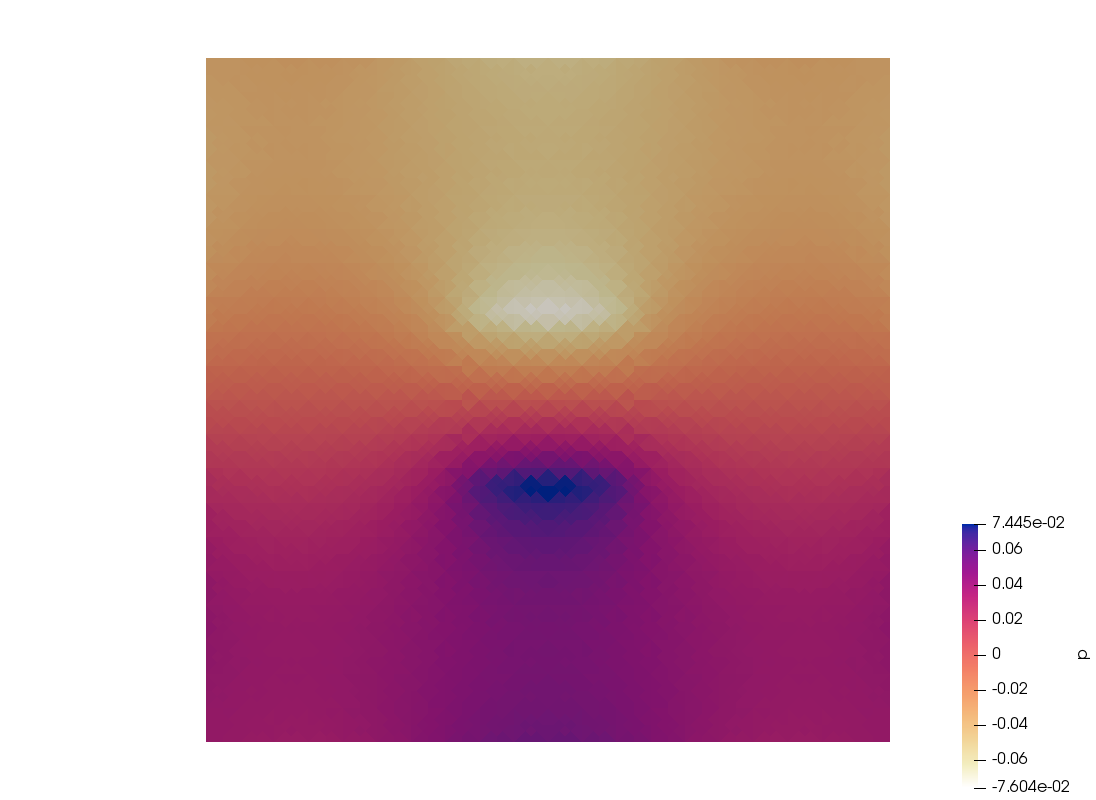
\includegraphics[width=3.8cm]{python_codes/fieldstone_78/results/block/reduced/p3}\\
{\captionfont buoyancy term $b_y$; pressure field for regular, Stenberg, Le Tallec, Qin \& Zhang.} 
\end{center}


%.....................................................
\paragraph{Results - sinking block - full density}

We then proceed with $\rho g_y=-1$ in the surrounding fluid and $\rho g_y=-1+\delta$ in the block.

\begin{center}
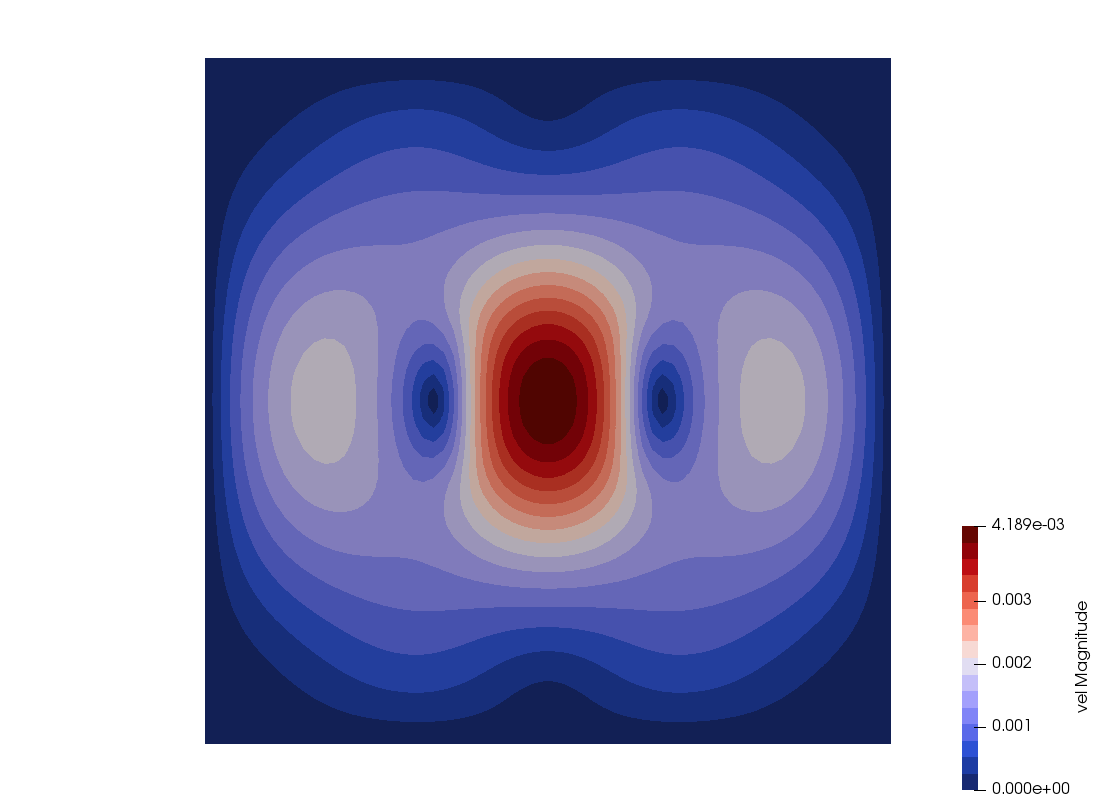
\includegraphics[width=3.8cm]{python_codes/fieldstone_78/results/block/full/vel0}
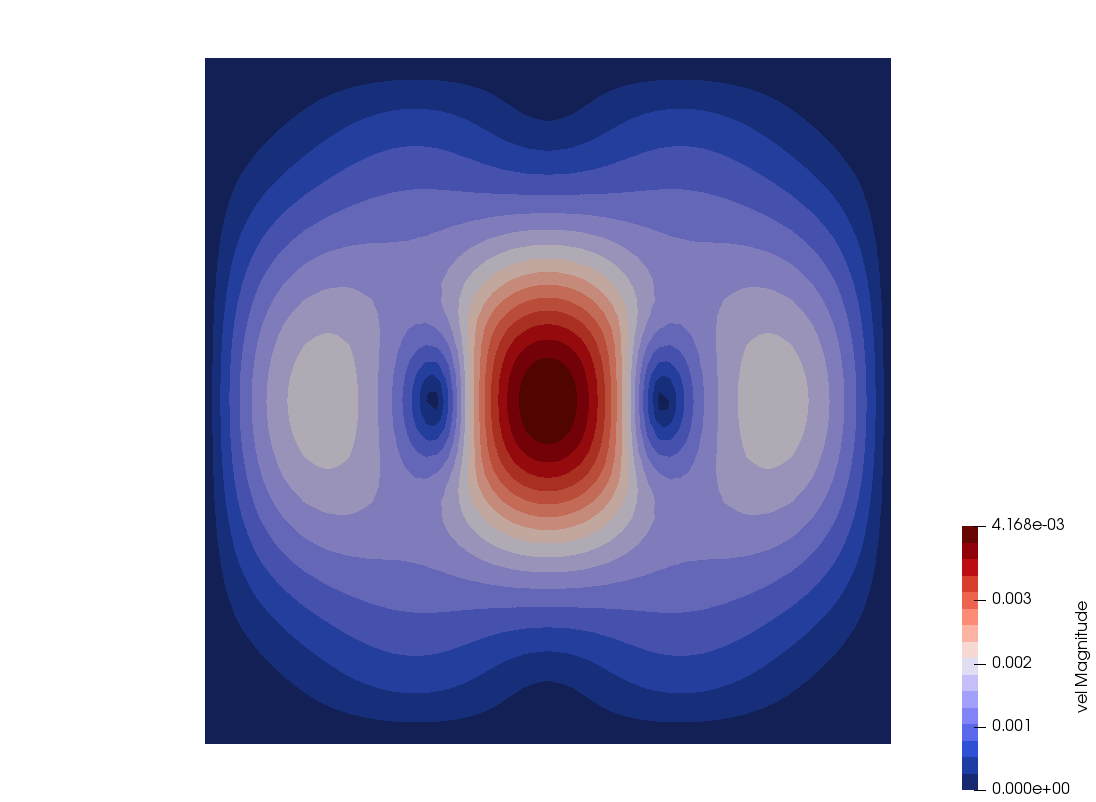
\includegraphics[width=3.8cm]{python_codes/fieldstone_78/results/block/full/vel1}
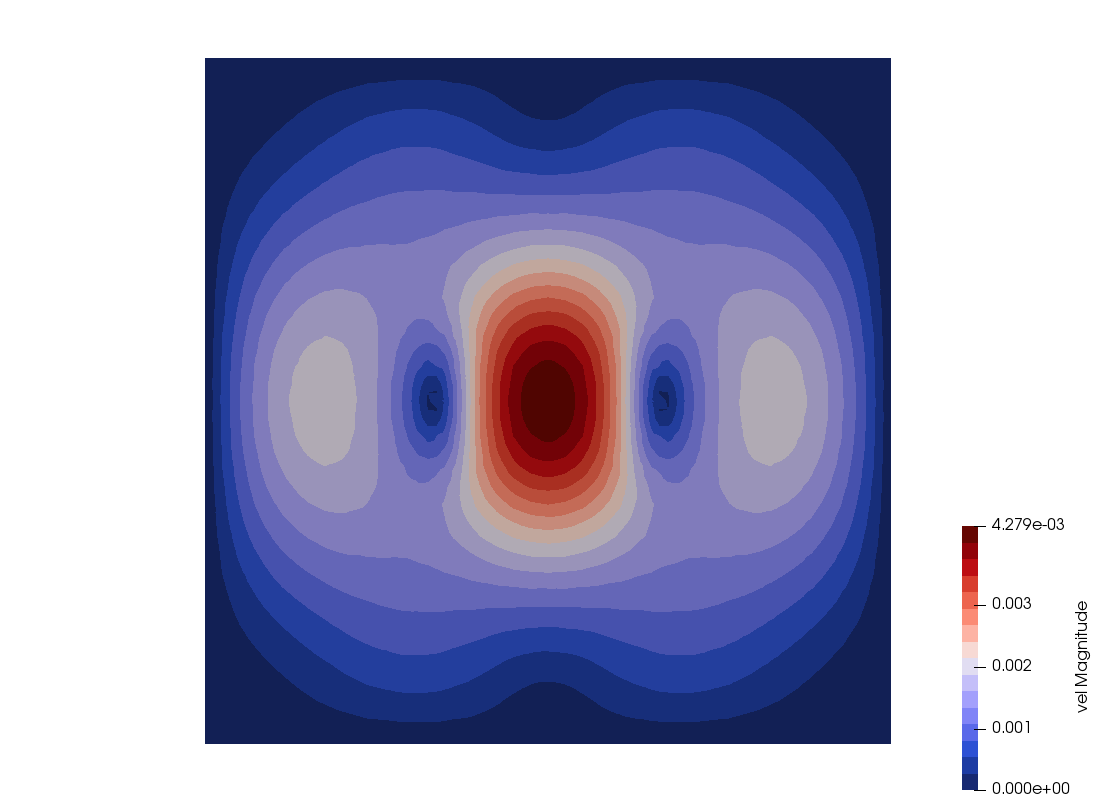
\includegraphics[width=3.8cm]{python_codes/fieldstone_78/results/block/full/vel2}
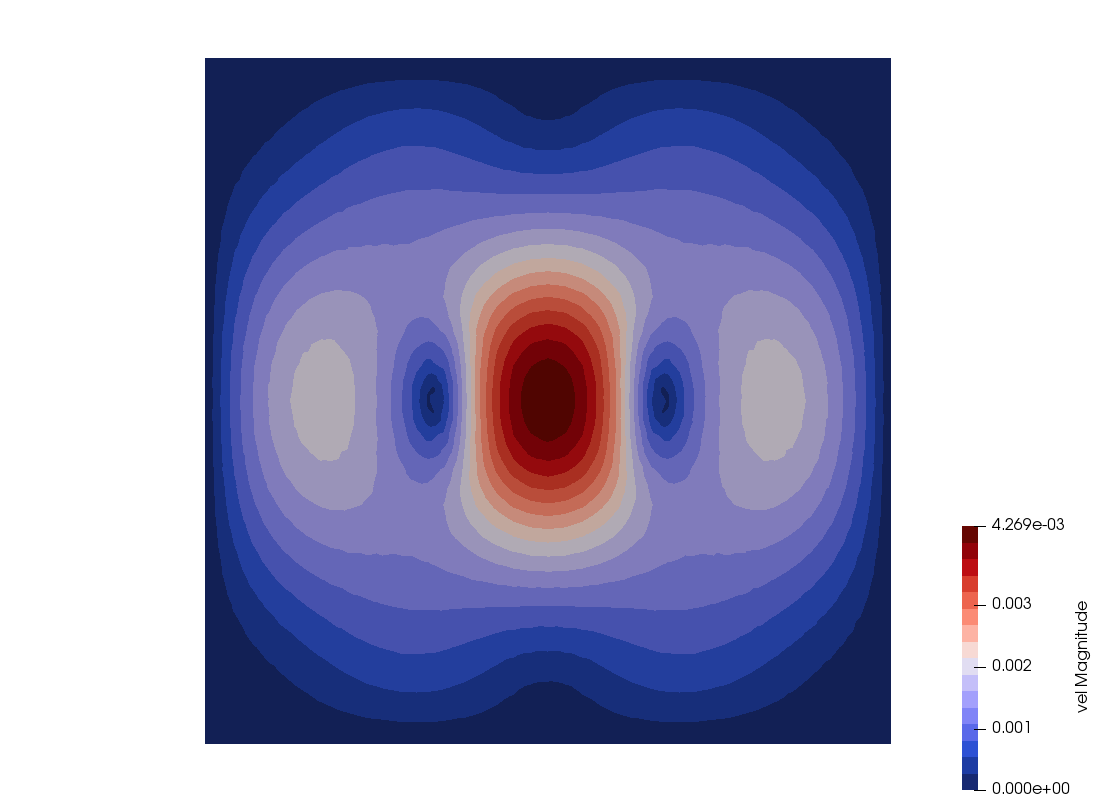
\includegraphics[width=3.8cm]{python_codes/fieldstone_78/results/block/full/vel3}\\
\includegraphics[width=3.8cm]{python_codes/fieldstone_78/results/block/full/p0}
\includegraphics[width=3.8cm]{python_codes/fieldstone_78/results/block/full/p1}
\includegraphics[width=3.8cm]{python_codes/fieldstone_78/results/block/full/p2}
\includegraphics[width=3.8cm]{python_codes/fieldstone_78/results/block/full/p3}\\
{\captionfont buoyancy term $b_y$; pressure field for regular, Stenberg, Le Tallec, Qin \& Zhang.} 
\end{center}













The velocity and presure fields are shown in the following figure for various values of $\delta$.
We see that when the density of the block approaches the one of the surrounding fluid the 
velocity field shows abnormal stripes while the pressure field looks hydrostatic.   

%\begin{center}
%\includegraphics[width=3.84cm]{python_codes/fieldstone_78/results/block/p_delta0p001}
%\includegraphics[width=3.84cm]{python_codes/fieldstone_78/results/block/p_delta0p01}
%\includegraphics[width=3.84cm]{python_codes/fieldstone_78/results/block/p_delta0p1}
%\includegraphics[width=3.84cm]{python_codes/fieldstone_78/results/block/p_delta1}\\
%\includegraphics[width=3.84cm]{python_codes/fieldstone_78/results/block/vel_delta0p001}
%\includegraphics[width=3.84cm]{python_codes/fieldstone_78/results/block/vel_delta0p01}
%\includegraphics[width=3.84cm]{python_codes/fieldstone_78/results/block/vel_delta0p1}
%\includegraphics[width=3.84cm]{python_codes/fieldstone_78/results/block/vel_delta1}\\
%{\captionfont Resolution 64x64. From left to right: $\delta=0.001,0.01,0.01,1$}
%\end{center}

\newpage
%..................................
\paragraph{Results - Stokes sphere}

This is the same experiment as above, except for the geometry of the object 
which is now a sphere of radius 0.125. Its density is 2 while the surrounding is 1.  
Its viscosity is $10^4$ while the surrounding is 1.

\begin{center}
\includegraphics[width=3.84cm]{python_codes/fieldstone_78/results/sphere/eta0}
\includegraphics[width=3.84cm]{python_codes/fieldstone_78/results/sphere/eta1}
\includegraphics[width=3.84cm]{python_codes/fieldstone_78/results/sphere/eta2}
\includegraphics[width=3.84cm]{python_codes/fieldstone_78/results/sphere/eta3}\\
\includegraphics[width=3.84cm]{python_codes/fieldstone_78/results/sphere/vel0}
\includegraphics[width=3.84cm]{python_codes/fieldstone_78/results/sphere/vel1}
\includegraphics[width=3.84cm]{python_codes/fieldstone_78/results/sphere/vel2}
\includegraphics[width=3.84cm]{python_codes/fieldstone_78/results/sphere/vel3}\\
\includegraphics[width=3.84cm]{python_codes/fieldstone_78/results/sphere/p0}
\includegraphics[width=3.84cm]{python_codes/fieldstone_78/results/sphere/p1}
\includegraphics[width=3.84cm]{python_codes/fieldstone_78/results/sphere/p2}
\includegraphics[width=3.84cm]{python_codes/fieldstone_78/results/sphere/p3}\\
\includegraphics[width=3.84cm]{python_codes/fieldstone_78/results/sphere/q0}
\includegraphics[width=3.84cm]{python_codes/fieldstone_78/results/sphere/q1}
\includegraphics[width=3.84cm]{python_codes/fieldstone_78/results/sphere/q2}
\includegraphics[width=3.84cm]{python_codes/fieldstone_78/results/sphere/q3}\\
{\captionfont From top to bottom: viscosity, velocity, elemental and nodal pressure fields. 
From left to right: regular, Stenberg, Le Tallec, Qin \& Zhang. Meshes with 5000 elements.}
\end{center}

\begin{center}
\includegraphics[width=10cm]{python_codes/fieldstone_78/results/sphere/vrms}
\end{center}

\begin{center}
\includegraphics[width=7cm]{python_codes/fieldstone_78/results/sphere/ustats}
\includegraphics[width=7cm]{python_codes/fieldstone_78/results/sphere/vstats}\\
\includegraphics[width=7cm]{python_codes/fieldstone_78/results/sphere/pstats}
\includegraphics[width=7cm]{python_codes/fieldstone_78/results/sphere/qstats}
\end{center}

All (macro-)elements converge to the same vrms and show very similar velocity and pressure statistics.
Stenberg is undeniably the best in terms of pressure under/over shoot. 



